% IEEE Access version of paper/manuscript.tex (format only; generated by scripts/make_ieee_version.py - do not edit by hand).
% Requires the official class files from the IEEE Access template (ieeeaccess.cls, spotcolor.sty, logo images); see README.txt.
\documentclass{ieeeaccess}
\usepackage{cite}
\usepackage{amsmath,amssymb,amsfonts}
\usepackage{graphicx}
\usepackage{textcomp}
\usepackage{booktabs,multirow,array,xcolor,url,placeins}
\urlstyle{tt}
\emergencystretch=2em
% let several wide floats share a page and let text and floats fill the pages (the defaults leave large gaps)
\setcounter{topnumber}{4}\setcounter{bottomnumber}{3}\setcounter{totalnumber}{8}\setcounter{dbltopnumber}{6}
\renewcommand{\topfraction}{0.9}\renewcommand{\bottomfraction}{0.8}\renewcommand{\textfraction}{0.1}
\renewcommand{\floatpagefraction}{0.7}\renewcommand{\dbltopfraction}{0.9}\renewcommand{\dblfloatpagefraction}{0.7}
% on float-only pages stack the floats from the top with a fixed gap instead of spreading them over the page
\makeatletter
\setlength{\@fptop}{0pt}\setlength{\@fpsep}{12pt}\setlength{\@fpbot}{0pt plus 1fil}
\setlength{\@dblfptop}{0pt}\setlength{\@dblfpsep}{12pt}\setlength{\@dblfpbot}{0pt plus 1fil}
\makeatother
\renewcommand{\arraystretch}{1.08}
\newsavebox{\fitboxbin}
% typeset a table at its natural width, scaled down only if it is wider than #1
\newcommand{\fitbox}[2]{\sbox{\fitboxbin}{#2}\ifdim\wd\fitboxbin>#1\resizebox{#1}{!}{\usebox{\fitboxbin}}\else\usebox{\fitboxbin}\fi}
% GENERATED by scripts/make_paper_assets.py -- do not edit by hand.
\newcommand{\AdpEceAllM}{0.060}
\newcommand{\AdpEceAllN}{3}
\newcommand{\AdpEceAllP}{0.060 $\pm$ 0.009}
\newcommand{\AdpEceAllS}{0.009}
\newcommand{\AdpEceAllZ}{0.050}
\newcommand{\AdpEceCasM}{0.112}
\newcommand{\AdpEceCasN}{3}
\newcommand{\AdpEceCasP}{0.112 $\pm$ 0.002}
\newcommand{\AdpEceCasS}{0.002}
\newcommand{\AdpEceCasZ}{0.111}
\newcommand{\AdpEceGdcM}{0.041}
\newcommand{\AdpEceGdcN}{3}
\newcommand{\AdpEceGdcP}{0.041 $\pm$ 0.002}
\newcommand{\AdpEceGdcS}{0.002}
\newcommand{\AdpEceGdcZ}{0.039}
\newcommand{\AdpEceHrgM}{0.051}
\newcommand{\AdpEceHrgN}{3}
\newcommand{\AdpEceHrgP}{0.051 $\pm$ 0.003}
\newcommand{\AdpEceHrgS}{0.003}
\newcommand{\AdpEceHrgZ}{0.050}
\newcommand{\AdpEceLfsM}{0.036}
\newcommand{\AdpEceLfsN}{3}
\newcommand{\AdpEceLfsP}{0.036 $\pm$ 0.029}
\newcommand{\AdpEceLfsS}{0.029}
\newcommand{\AdpEceLfsZ}{0.004}
\newcommand{\AdpEceLmhM}{0.058}
\newcommand{\AdpEceLmhN}{3}
\newcommand{\AdpEceLmhP}{0.058 $\pm$ 0.016}
\newcommand{\AdpEceLmhS}{0.016}
\newcommand{\AdpEceLmhZ}{0.044}
\newcommand{\AdpFoneAllM}{37.5}
\newcommand{\AdpFoneAllN}{3}
\newcommand{\AdpFoneAllP}{37.5 $\pm$ 2.6}
\newcommand{\AdpFoneAllS}{2.6}
\newcommand{\AdpFoneAllZ}{40.1}
\newcommand{\AdpFoneCasM}{30.1}
\newcommand{\AdpFoneCasN}{3}
\newcommand{\AdpFoneCasP}{30.1 $\pm$ 3.6}
\newcommand{\AdpFoneCasS}{3.6}
\newcommand{\AdpFoneCasZ}{34.1}
\newcommand{\AdpFoneGdcM}{45.6}
\newcommand{\AdpFoneGdcN}{3}
\newcommand{\AdpFoneGdcP}{45.6 $\pm$ 1.0}
\newcommand{\AdpFoneGdcS}{1.0}
\newcommand{\AdpFoneGdcZ}{44.8}
\newcommand{\AdpFoneHrgM}{56.5}
\newcommand{\AdpFoneHrgN}{3}
\newcommand{\AdpFoneHrgP}{56.5 $\pm$ 1.7}
\newcommand{\AdpFoneHrgS}{1.7}
\newcommand{\AdpFoneHrgZ}{58.3}
\newcommand{\AdpFoneLfsM}{22.8}
\newcommand{\AdpFoneLfsN}{3}
\newcommand{\AdpFoneLfsP}{22.8 $\pm$ 8.7}
\newcommand{\AdpFoneLfsS}{8.7}
\newcommand{\AdpFoneLfsZ}{32.7}
\newcommand{\AdpFoneLmhM}{32.2}
\newcommand{\AdpFoneLmhN}{3}
\newcommand{\AdpFoneLmhP}{32.2 $\pm$ 4.5}
\newcommand{\AdpFoneLmhS}{4.5}
\newcommand{\AdpFoneLmhZ}{30.7}
\newcommand{\AdpIouAllM}{23.8}
\newcommand{\AdpIouAllN}{3}
\newcommand{\AdpIouAllP}{23.8 $\pm$ 1.8}
\newcommand{\AdpIouAllS}{1.8}
\newcommand{\AdpIouAllZ}{25.6}
\newcommand{\AdpIouCasM}{17.8}
\newcommand{\AdpIouCasN}{3}
\newcommand{\AdpIouCasP}{17.8 $\pm$ 2.5}
\newcommand{\AdpIouCasS}{2.5}
\newcommand{\AdpIouCasZ}{20.6}
\newcommand{\AdpIouGdcM}{29.6}
\newcommand{\AdpIouGdcN}{3}
\newcommand{\AdpIouGdcP}{29.6 $\pm$ 0.8}
\newcommand{\AdpIouGdcS}{0.8}
\newcommand{\AdpIouGdcZ}{28.9}
\newcommand{\AdpIouHrgM}{39.4}
\newcommand{\AdpIouHrgN}{3}
\newcommand{\AdpIouHrgP}{39.4 $\pm$ 1.7}
\newcommand{\AdpIouHrgS}{1.7}
\newcommand{\AdpIouHrgZ}{41.1}
\newcommand{\AdpIouLfsM}{13.0}
\newcommand{\AdpIouLfsN}{3}
\newcommand{\AdpIouLfsP}{13.0 $\pm$ 5.7}
\newcommand{\AdpIouLfsS}{5.7}
\newcommand{\AdpIouLfsZ}{19.5}
\newcommand{\AdpIouLmhM}{19.3}
\newcommand{\AdpIouLmhN}{3}
\newcommand{\AdpIouLmhP}{19.3 $\pm$ 3.2}
\newcommand{\AdpIouLmhS}{3.2}
\newcommand{\AdpIouLmhZ}{18.1}
\newcommand{\AdpMiouAllM}{57.0}
\newcommand{\AdpMiouAllN}{3}
\newcommand{\AdpMiouAllP}{57.0 $\pm$ 1.3}
\newcommand{\AdpMiouAllS}{1.3}
\newcommand{\AdpMiouAllZ}{58.4}
\newcommand{\AdpMiouCasM}{51.9}
\newcommand{\AdpMiouCasN}{3}
\newcommand{\AdpMiouCasP}{51.9 $\pm$ 1.0}
\newcommand{\AdpMiouCasS}{1.0}
\newcommand{\AdpMiouCasZ}{53.0}
\newcommand{\AdpMiouGdcM}{61.6}
\newcommand{\AdpMiouGdcN}{3}
\newcommand{\AdpMiouGdcP}{61.6 $\pm$ 0.4}
\newcommand{\AdpMiouGdcS}{0.4}
\newcommand{\AdpMiouGdcZ}{61.3}
\newcommand{\AdpMiouHrgM}{65.8}
\newcommand{\AdpMiouHrgN}{3}
\newcommand{\AdpMiouHrgP}{65.8 $\pm$ 0.8}
\newcommand{\AdpMiouHrgS}{0.8}
\newcommand{\AdpMiouHrgZ}{66.6}
\newcommand{\AdpMiouLfsM}{51.2}
\newcommand{\AdpMiouLfsN}{3}
\newcommand{\AdpMiouLfsP}{51.2 $\pm$ 4.7}
\newcommand{\AdpMiouLfsS}{4.7}
\newcommand{\AdpMiouLfsZ}{56.6}
\newcommand{\AdpMiouLmhM}{54.5}
\newcommand{\AdpMiouLmhN}{3}
\newcommand{\AdpMiouLmhP}{54.5 $\pm$ 0.4}
\newcommand{\AdpMiouLmhS}{0.4}
\newcommand{\AdpMiouLmhZ}{54.7}
\newcommand{\AdpPrAllM}{0.439}
\newcommand{\AdpPrAllN}{3}
\newcommand{\AdpPrAllP}{0.439 $\pm$ 0.032}
\newcommand{\AdpPrAllS}{0.032}
\newcommand{\AdpPrAllZ}{0.476}
\newcommand{\AdpPrCasM}{0.427}
\newcommand{\AdpPrCasN}{3}
\newcommand{\AdpPrCasP}{0.427 $\pm$ 0.018}
\newcommand{\AdpPrCasS}{0.018}
\newcommand{\AdpPrCasZ}{0.406}
\newcommand{\AdpPrGdcM}{0.516}
\newcommand{\AdpPrGdcN}{3}
\newcommand{\AdpPrGdcP}{0.516 $\pm$ 0.007}
\newcommand{\AdpPrGdcS}{0.007}
\newcommand{\AdpPrGdcZ}{0.509}
\newcommand{\AdpPrHrgM}{0.630}
\newcommand{\AdpPrHrgN}{3}
\newcommand{\AdpPrHrgP}{0.630 $\pm$ 0.015}
\newcommand{\AdpPrHrgS}{0.015}
\newcommand{\AdpPrHrgZ}{0.646}
\newcommand{\AdpPrLfsM}{0.267}
\newcommand{\AdpPrLfsN}{3}
\newcommand{\AdpPrLfsP}{0.267 $\pm$ 0.147}
\newcommand{\AdpPrLfsS}{0.147}
\newcommand{\AdpPrLfsZ}{0.427}
\newcommand{\AdpPrLmhM}{0.356}
\newcommand{\AdpPrLmhN}{3}
\newcommand{\AdpPrLmhP}{0.356 $\pm$ 0.054}
\newcommand{\AdpPrLmhS}{0.054}
\newcommand{\AdpPrLmhZ}{0.391}
\newcommand{\AdpPrecAllM}{51.5}
\newcommand{\AdpPrecAllN}{3}
\newcommand{\AdpPrecAllP}{51.5 $\pm$ 2.1}
\newcommand{\AdpPrecAllS}{2.1}
\newcommand{\AdpPrecAllZ}{53.0}
\newcommand{\AdpPrecCasM}{61.0}
\newcommand{\AdpPrecCasN}{3}
\newcommand{\AdpPrecCasP}{61.0 $\pm$ 6.6}
\newcommand{\AdpPrecCasS}{6.6}
\newcommand{\AdpPrecCasZ}{53.9}
\newcommand{\AdpPrecGdcM}{65.1}
\newcommand{\AdpPrecGdcN}{3}
\newcommand{\AdpPrecGdcP}{65.1 $\pm$ 2.6}
\newcommand{\AdpPrecGdcS}{2.6}
\newcommand{\AdpPrecGdcZ}{66.7}
\newcommand{\AdpPrecHrgM}{70.3}
\newcommand{\AdpPrecHrgN}{3}
\newcommand{\AdpPrecHrgP}{70.3 $\pm$ 2.2}
\newcommand{\AdpPrecHrgS}{2.2}
\newcommand{\AdpPrecHrgZ}{68.0}
\newcommand{\AdpPrecLfsM}{14.1}
\newcommand{\AdpPrecLfsN}{3}
\newcommand{\AdpPrecLfsP}{14.1 $\pm$ 6.4}
\newcommand{\AdpPrecLfsS}{6.4}
\newcommand{\AdpPrecLfsZ}{21.4}
\newcommand{\AdpPrecLmhM}{47.2}
\newcommand{\AdpPrecLmhN}{3}
\newcommand{\AdpPrecLmhP}{47.2 $\pm$ 12.3}
\newcommand{\AdpPrecLmhS}{12.3}
\newcommand{\AdpPrecLmhZ}{54.8}
\newcommand{\AdpRecAllM}{38.9}
\newcommand{\AdpRecAllN}{3}
\newcommand{\AdpRecAllP}{38.9 $\pm$ 3.1}
\newcommand{\AdpRecAllS}{3.1}
\newcommand{\AdpRecAllZ}{39.9}
\newcommand{\AdpRecCasM}{20.3}
\newcommand{\AdpRecCasN}{3}
\newcommand{\AdpRecCasP}{20.3 $\pm$ 4.1}
\newcommand{\AdpRecCasS}{4.1}
\newcommand{\AdpRecCasZ}{24.9}
\newcommand{\AdpRecGdcM}{35.2}
\newcommand{\AdpRecGdcN}{3}
\newcommand{\AdpRecGdcP}{35.2 $\pm$ 1.9}
\newcommand{\AdpRecGdcS}{1.9}
\newcommand{\AdpRecGdcZ}{33.7}
\newcommand{\AdpRecHrgM}{47.4}
\newcommand{\AdpRecHrgN}{3}
\newcommand{\AdpRecHrgP}{47.4 $\pm$ 3.2}
\newcommand{\AdpRecHrgS}{3.2}
\newcommand{\AdpRecHrgZ}{51.0}
\newcommand{\AdpRecLfsM}{63.7}
\newcommand{\AdpRecLfsN}{3}
\newcommand{\AdpRecLfsP}{63.7 $\pm$ 4.9}
\newcommand{\AdpRecLfsS}{4.9}
\newcommand{\AdpRecLfsZ}{68.8}
\newcommand{\AdpRecLmhM}{28.0}
\newcommand{\AdpRecLmhN}{3}
\newcommand{\AdpRecLmhP}{28.0 $\pm$ 13.1}
\newcommand{\AdpRecLmhS}{13.1}
\newcommand{\AdpRecLmhZ}{21.3}
\newcommand{\CeilIou}{89.5}
\newcommand{\CeilMiou}{94.7}
\newcommand{\CompEceAllM}{0.061}
\newcommand{\CompEceAllN}{3}
\newcommand{\CompEceAllP}{0.061 $\pm$ 0.012}
\newcommand{\CompEceAllS}{0.012}
\newcommand{\CompEceAllZ}{0.075}
\newcommand{\CompEceCasM}{0.107}
\newcommand{\CompEceCasN}{3}
\newcommand{\CompEceCasP}{0.107 $\pm$ 0.003}
\newcommand{\CompEceCasS}{0.003}
\newcommand{\CompEceCasZ}{0.105}
\newcommand{\CompEceGdcM}{0.027}
\newcommand{\CompEceGdcN}{3}
\newcommand{\CompEceGdcP}{0.027 $\pm$ 0.001}
\newcommand{\CompEceGdcS}{0.001}
\newcommand{\CompEceGdcZ}{0.026}
\newcommand{\CompEceHrgM}{0.052}
\newcommand{\CompEceHrgN}{3}
\newcommand{\CompEceHrgP}{0.052 $\pm$ 0.001}
\newcommand{\CompEceHrgS}{0.001}
\newcommand{\CompEceHrgZ}{0.053}
\newcommand{\CompEceLfsM}{0.030}
\newcommand{\CompEceLfsN}{3}
\newcommand{\CompEceLfsP}{0.030 $\pm$ 0.028}
\newcommand{\CompEceLfsS}{0.028}
\newcommand{\CompEceLfsZ}{0.060}
\newcommand{\CompEceLmhM}{0.090}
\newcommand{\CompEceLmhN}{3}
\newcommand{\CompEceLmhP}{0.090 $\pm$ 0.037}
\newcommand{\CompEceLmhS}{0.037}
\newcommand{\CompEceLmhZ}{0.133}
\newcommand{\CompFoneAllM}{42.6}
\newcommand{\CompFoneAllN}{3}
\newcommand{\CompFoneAllP}{42.6 $\pm$ 3.3}
\newcommand{\CompFoneAllS}{3.3}
\newcommand{\CompFoneAllZ}{39.3}
\newcommand{\CompFoneCasM}{43.4}
\newcommand{\CompFoneCasN}{3}
\newcommand{\CompFoneCasP}{43.4 $\pm$ 2.1}
\newcommand{\CompFoneCasS}{2.1}
\newcommand{\CompFoneCasZ}{43.4}
\newcommand{\CompFoneGdcM}{62.4}
\newcommand{\CompFoneGdcN}{3}
\newcommand{\CompFoneGdcP}{62.4 $\pm$ 0.6}
\newcommand{\CompFoneGdcS}{0.6}
\newcommand{\CompFoneGdcZ}{62.0}
\newcommand{\CompFoneHrgM}{54.8}
\newcommand{\CompFoneHrgN}{3}
\newcommand{\CompFoneHrgP}{54.8 $\pm$ 0.8}
\newcommand{\CompFoneHrgS}{0.8}
\newcommand{\CompFoneHrgZ}{53.9}
\newcommand{\CompFoneLfsM}{24.9}
\newcommand{\CompFoneLfsN}{3}
\newcommand{\CompFoneLfsP}{24.9 $\pm$ 11.5}
\newcommand{\CompFoneLfsS}{11.5}
\newcommand{\CompFoneLfsZ}{14.4}
\newcommand{\CompFoneLmhM}{27.6}
\newcommand{\CompFoneLmhN}{3}
\newcommand{\CompFoneLmhP}{27.6 $\pm$ 4.3}
\newcommand{\CompFoneLmhS}{4.3}
\newcommand{\CompFoneLmhZ}{22.6}
\newcommand{\CompIouAllM}{28.3}
\newcommand{\CompIouAllN}{3}
\newcommand{\CompIouAllP}{28.3 $\pm$ 2.3}
\newcommand{\CompIouAllS}{2.3}
\newcommand{\CompIouAllZ}{26.0}
\newcommand{\CompIouCasM}{27.7}
\newcommand{\CompIouCasN}{3}
\newcommand{\CompIouCasP}{27.7 $\pm$ 1.7}
\newcommand{\CompIouCasS}{1.7}
\newcommand{\CompIouCasZ}{27.7}
\newcommand{\CompIouGdcM}{45.3}
\newcommand{\CompIouGdcN}{3}
\newcommand{\CompIouGdcP}{45.3 $\pm$ 0.6}
\newcommand{\CompIouGdcS}{0.6}
\newcommand{\CompIouGdcZ}{45.0}
\newcommand{\CompIouHrgM}{37.7}
\newcommand{\CompIouHrgN}{3}
\newcommand{\CompIouHrgP}{37.7 $\pm$ 0.7}
\newcommand{\CompIouHrgS}{0.7}
\newcommand{\CompIouHrgZ}{36.9}
\newcommand{\CompIouLfsM}{14.5}
\newcommand{\CompIouLfsN}{3}
\newcommand{\CompIouLfsP}{14.5 $\pm$ 7.6}
\newcommand{\CompIouLfsS}{7.6}
\newcommand{\CompIouLfsZ}{7.7}
\newcommand{\CompIouLmhM}{16.0}
\newcommand{\CompIouLmhN}{3}
\newcommand{\CompIouLmhP}{16.0 $\pm$ 2.9}
\newcommand{\CompIouLmhS}{2.9}
\newcommand{\CompIouLmhZ}{12.8}
\newcommand{\CompMiouAllM}{58.9}
\newcommand{\CompMiouAllN}{3}
\newcommand{\CompMiouAllP}{58.9 $\pm$ 1.8}
\newcommand{\CompMiouAllS}{1.8}
\newcommand{\CompMiouAllZ}{57.0}
\newcommand{\CompMiouCasM}{56.8}
\newcommand{\CompMiouCasN}{3}
\newcommand{\CompMiouCasP}{56.8 $\pm$ 0.8}
\newcommand{\CompMiouCasS}{0.8}
\newcommand{\CompMiouCasZ}{57.0}
\newcommand{\CompMiouGdcM}{69.7}
\newcommand{\CompMiouGdcN}{3}
\newcommand{\CompMiouGdcP}{69.7 $\pm$ 0.5}
\newcommand{\CompMiouGdcS}{0.5}
\newcommand{\CompMiouGdcZ}{69.4}
\newcommand{\CompMiouHrgM}{64.7}
\newcommand{\CompMiouHrgN}{3}
\newcommand{\CompMiouHrgP}{64.7 $\pm$ 0.5}
\newcommand{\CompMiouHrgS}{0.5}
\newcommand{\CompMiouHrgZ}{64.2}
\newcommand{\CompMiouLfsM}{52.9}
\newcommand{\CompMiouLfsN}{3}
\newcommand{\CompMiouLfsP}{52.9 $\pm$ 5.8}
\newcommand{\CompMiouLfsS}{5.8}
\newcommand{\CompMiouLfsZ}{47.8}
\newcommand{\CompMiouLmhM}{50.3}
\newcommand{\CompMiouLmhN}{3}
\newcommand{\CompMiouLmhP}{50.3 $\pm$ 3.1}
\newcommand{\CompMiouLmhS}{3.1}
\newcommand{\CompMiouLmhZ}{46.7}
\newcommand{\CompPrAllM}{0.429}
\newcommand{\CompPrAllN}{3}
\newcommand{\CompPrAllP}{0.429 $\pm$ 0.032}
\newcommand{\CompPrAllS}{0.032}
\newcommand{\CompPrAllZ}{0.395}
\newcommand{\CompPrCasM}{0.448}
\newcommand{\CompPrCasN}{3}
\newcommand{\CompPrCasP}{0.448 $\pm$ 0.013}
\newcommand{\CompPrCasS}{0.013}
\newcommand{\CompPrCasZ}{0.461}
\newcommand{\CompPrGdcM}{0.657}
\newcommand{\CompPrGdcN}{3}
\newcommand{\CompPrGdcP}{0.657 $\pm$ 0.017}
\newcommand{\CompPrGdcS}{0.017}
\newcommand{\CompPrGdcZ}{0.644}
\newcommand{\CompPrHrgM}{0.595}
\newcommand{\CompPrHrgN}{3}
\newcommand{\CompPrHrgP}{0.595 $\pm$ 0.011}
\newcommand{\CompPrHrgS}{0.011}
\newcommand{\CompPrHrgZ}{0.586}
\newcommand{\CompPrLfsM}{0.215}
\newcommand{\CompPrLfsN}{3}
\newcommand{\CompPrLfsP}{0.215 $\pm$ 0.111}
\newcommand{\CompPrLfsS}{0.111}
\newcommand{\CompPrLfsZ}{0.105}
\newcommand{\CompPrLmhM}{0.232}
\newcommand{\CompPrLmhN}{3}
\newcommand{\CompPrLmhP}{0.232 $\pm$ 0.044}
\newcommand{\CompPrLmhS}{0.044}
\newcommand{\CompPrLmhZ}{0.181}
\newcommand{\CompPrecAllM}{45.3}
\newcommand{\CompPrecAllN}{3}
\newcommand{\CompPrecAllP}{45.3 $\pm$ 3.2}
\newcommand{\CompPrecAllS}{3.2}
\newcommand{\CompPrecAllZ}{41.8}
\newcommand{\CompPrecCasM}{55.9}
\newcommand{\CompPrecCasN}{3}
\newcommand{\CompPrecCasP}{55.9 $\pm$ 2.8}
\newcommand{\CompPrecCasS}{2.8}
\newcommand{\CompPrecCasZ}{59.1}
\newcommand{\CompPrecGdcM}{62.3}
\newcommand{\CompPrecGdcN}{3}
\newcommand{\CompPrecGdcP}{62.3 $\pm$ 4.1}
\newcommand{\CompPrecGdcS}{4.1}
\newcommand{\CompPrecGdcZ}{59.0}
\newcommand{\CompPrecHrgM}{66.5}
\newcommand{\CompPrecHrgN}{3}
\newcommand{\CompPrecHrgP}{66.5 $\pm$ 2.3}
\newcommand{\CompPrecHrgS}{2.3}
\newcommand{\CompPrecHrgZ}{64.7}
\newcommand{\CompPrecLfsM}{16.6}
\newcommand{\CompPrecLfsN}{3}
\newcommand{\CompPrecLfsP}{16.6 $\pm$ 9.6}
\newcommand{\CompPrecLfsS}{9.6}
\newcommand{\CompPrecLfsZ}{8.5}
\newcommand{\CompPrecLmhM}{25.0}
\newcommand{\CompPrecLmhN}{3}
\newcommand{\CompPrecLmhP}{25.0 $\pm$ 6.2}
\newcommand{\CompPrecLmhS}{6.2}
\newcommand{\CompPrecLmhZ}{17.8}
\newcommand{\CompRecAllM}{46.5}
\newcommand{\CompRecAllN}{3}
\newcommand{\CompRecAllP}{46.5 $\pm$ 1.9}
\newcommand{\CompRecAllS}{1.9}
\newcommand{\CompRecAllZ}{44.3}
\newcommand{\CompRecCasM}{35.7}
\newcommand{\CompRecCasN}{3}
\newcommand{\CompRecCasP}{35.7 $\pm$ 3.3}
\newcommand{\CompRecCasS}{3.3}
\newcommand{\CompRecCasZ}{34.3}
\newcommand{\CompRecGdcM}{62.7}
\newcommand{\CompRecGdcN}{3}
\newcommand{\CompRecGdcP}{62.7 $\pm$ 2.9}
\newcommand{\CompRecGdcS}{2.9}
\newcommand{\CompRecGdcZ}{65.4}
\newcommand{\CompRecHrgM}{46.6}
\newcommand{\CompRecHrgN}{3}
\newcommand{\CompRecHrgP}{46.6 $\pm$ 0.7}
\newcommand{\CompRecHrgS}{0.7}
\newcommand{\CompRecHrgZ}{46.2}
\newcommand{\CompRecLfsM}{56.0}
\newcommand{\CompRecLfsN}{3}
\newcommand{\CompRecLfsP}{56.0 $\pm$ 10.0}
\newcommand{\CompRecLfsS}{10.0}
\newcommand{\CompRecLfsZ}{45.1}
\newcommand{\CompRecLmhM}{31.6}
\newcommand{\CompRecLmhN}{3}
\newcommand{\CompRecLmhP}{31.6 $\pm$ 2.4}
\newcommand{\CompRecLmhS}{2.4}
\newcommand{\CompRecLmhZ}{30.9}
\newcommand{\DiffAdpSegCas}{$-$3.5}
\newcommand{\DiffAdpSegCnt}{5}
\newcommand{\DiffAdpSegGdc}{+1.0}
\newcommand{\DiffAdpSegHrg}{+2.5}
\newcommand{\DiffAdpSegLfs}{$-$0.3}
\newcommand{\DiffAdpSegLmh}{$-$2.5}
\newcommand{\DiffAdpSegMean}{$-$0.5}
\newcommand{\DiffAdpSegPos}{2}
\newcommand{\DiffKdSegCas}{$-$6.1}
\newcommand{\DiffKdSegCnt}{5}
\newcommand{\DiffKdSegGdc}{$-$1.1}
\newcommand{\DiffKdSegHrg}{$-$3.1}
\newcommand{\DiffKdSegLfs}{$-$3.7}
\newcommand{\DiffKdSegLmh}{+8.3}
\newcommand{\DiffKdSegMean}{$-$1.1}
\newcommand{\DiffKdSegPos}{1}
\newcommand{\DiffSegUnetCas}{+17.3}
\newcommand{\DiffSegUnetCnt}{5}
\newcommand{\DiffSegUnetGdc}{+10.7}
\newcommand{\DiffSegUnetHrg}{+6.5}
\newcommand{\DiffSegUnetLfs}{$-$4.4}
\newcommand{\DiffSegUnetLmh}{+4.3}
\newcommand{\DiffSegUnetMean}{+6.9}
\newcommand{\DiffSegUnetPos}{4}
\newcommand{\EvAllFive}{1}
\newcommand{\EvThreePlus}{5}
\newcommand{\EvTotal}{24}
\newcommand{\EvTwoPlus}{10}
\newcommand{\ExBestIouMax}{0.98}
\newcommand{\ExBestIouMin}{0.93}
\newcommand{\ExWorstIouMax}{0.00}
\newcommand{\ExWorstMaxPct}{5.2}
\newcommand{\ExWorstMinPct}{1.0}
\newcommand{\GdcOursMinusEssdTestMiou}{$-$2.7}
\newcommand{\GdcOursMinusEssdTestMioutwo}{$-$2.7}
\newcommand{\GdcValTestDeeplabGap}{34.5}
\newcommand{\GdcValTestSegGap}{29.2}
\newcommand{\GdcValTestUnetGap}{30.8}
\newcommand{\GflAdpPxOneTwoEight}{0.43}
\newcommand{\GflAdpPxTwoFiveSix}{1.75}
\newcommand{\GflDeeplabPxOneTwoEight}{1.97}
\newcommand{\GflDeeplabPxTwoFiveSix}{7.89}
\newcommand{\GflSegPxOneTwoEight}{0.42}
\newcommand{\GflSegPxTwoFiveSix}{1.75}
\newcommand{\GflTeachPxOneTwoEight}{2.26}
\newcommand{\GflTeachPxTwoFiveSix}{9.31}
\newcommand{\GflUnetPxOneTwoEight}{1.96}
\newcommand{\GflUnetPxTwoFiveSix}{7.82}
\newcommand{\InGdcRgbDeeplabBestEpoch}{19}
\newcommand{\InGdcRgbDeeplabBgIou}{99.1}
\newcommand{\InGdcRgbDeeplabEce}{0.005}
\newcommand{\InGdcRgbDeeplabFone}{51.7}
\newcommand{\InGdcRgbDeeplabGflops}{7.9}
\newcommand{\InGdcRgbDeeplabIou}{34.8}
\newcommand{\InGdcRgbDeeplabMacroFone}{75.6}
\newcommand{\InGdcRgbDeeplabMiou}{67.0}
\newcommand{\InGdcRgbDeeplabParamsM}{22.4}
\newcommand{\InGdcRgbDeeplabPr}{0.562}
\newcommand{\InGdcRgbDeeplabPrec}{63.2}
\newcommand{\InGdcRgbDeeplabRec}{43.7}
\newcommand{\InGdcRgbDeeplabValIou}{69.3}
\newcommand{\InGdcRgbSegBestEpoch}{19}
\newcommand{\InGdcRgbSegBgIou}{99.3}
\newcommand{\InGdcRgbSegEce}{0.004}
\newcommand{\InGdcRgbSegFone}{58.1}
\newcommand{\InGdcRgbSegGflops}{1.7}
\newcommand{\InGdcRgbSegIou}{40.9}
\newcommand{\InGdcRgbSegMacroFone}{78.9}
\newcommand{\InGdcRgbSegMiou}{70.1}
\newcommand{\InGdcRgbSegParamsM}{3.7}
\newcommand{\InGdcRgbSegPr}{0.654}
\newcommand{\InGdcRgbSegPrec}{72.6}
\newcommand{\InGdcRgbSegRec}{48.4}
\newcommand{\InGdcRgbSegValIou}{70.2}
\newcommand{\InGdcRgbSixtySegBestEpoch}{59}
\newcommand{\InGdcRgbSixtySegBgIou}{99.1}
\newcommand{\InGdcRgbSixtySegEce}{0.005}
\newcommand{\InGdcRgbSixtySegFone}{57.1}
\newcommand{\InGdcRgbSixtySegGflops}{1.7}
\newcommand{\InGdcRgbSixtySegIou}{40.0}
\newcommand{\InGdcRgbSixtySegMacroFone}{78.4}
\newcommand{\InGdcRgbSixtySegMiou}{69.6}
\newcommand{\InGdcRgbSixtySegParamsM}{3.7}
\newcommand{\InGdcRgbSixtySegPr}{0.529}
\newcommand{\InGdcRgbSixtySegPrec}{61.2}
\newcommand{\InGdcRgbSixtySegRec}{53.6}
\newcommand{\InGdcRgbSixtySegValIou}{71.6}
\newcommand{\InGdcRgbUnetBestEpoch}{17}
\newcommand{\InGdcRgbUnetBgIou}{99.2}
\newcommand{\InGdcRgbUnetEce}{0.005}
\newcommand{\InGdcRgbUnetFone}{55.8}
\newcommand{\InGdcRgbUnetGflops}{7.8}
\newcommand{\InGdcRgbUnetIou}{38.7}
\newcommand{\InGdcRgbUnetMacroFone}{77.7}
\newcommand{\InGdcRgbUnetMiou}{69.0}
\newcommand{\InGdcRgbUnetParamsM}{24.4}
\newcommand{\InGdcRgbUnetPr}{0.604}
\newcommand{\InGdcRgbUnetPrec}{68.5}
\newcommand{\InGdcRgbUnetRec}{47.1}
\newcommand{\InGdcRgbUnetValIou}{69.5}
\newcommand{\InLfsBankAdpBestEpoch}{5}
\newcommand{\InLfsBankAdpBgIou}{98.2}
\newcommand{\InLfsBankAdpEce}{0.011}
\newcommand{\InLfsBankAdpFone}{59.4}
\newcommand{\InLfsBankAdpGflops}{0.4}
\newcommand{\InLfsBankAdpIou}{42.2}
\newcommand{\InLfsBankAdpMacroFone}{79.2}
\newcommand{\InLfsBankAdpMiou}{70.2}
\newcommand{\InLfsBankAdpParamsM}{3.7}
\newcommand{\InLfsBankAdpPr}{0.604}
\newcommand{\InLfsBankAdpPrec}{51.5}
\newcommand{\InLfsBankAdpRec}{70.2}
\newcommand{\InLfsBankAdpValIou}{44.5}
\newcommand{\InLfsFourteenDeeplabBestEpoch}{41}
\newcommand{\InLfsFourteenDeeplabBgIou}{98.5}
\newcommand{\InLfsFourteenDeeplabEce}{0.011}
\newcommand{\InLfsFourteenDeeplabFone}{62.3}
\newcommand{\InLfsFourteenDeeplabGflops}{2.1}
\newcommand{\InLfsFourteenDeeplabIou}{45.3}
\newcommand{\InLfsFourteenDeeplabMacroFone}{80.8}
\newcommand{\InLfsFourteenDeeplabMiou}{71.9}
\newcommand{\InLfsFourteenDeeplabParamsM}{22.5}
\newcommand{\InLfsFourteenDeeplabPr}{0.636}
\newcommand{\InLfsFourteenDeeplabPrec}{58.3}
\newcommand{\InLfsFourteenDeeplabRec}{66.9}
\newcommand{\InLfsFourteenDeeplabValIou}{46.2}
\newcommand{\InLfsFourteenSegBestEpoch}{38}
\newcommand{\InLfsFourteenSegBgIou}{98.4}
\newcommand{\InLfsFourteenSegEce}{0.010}
\newcommand{\InLfsFourteenSegFone}{63.7}
\newcommand{\InLfsFourteenSegGflops}{0.4}
\newcommand{\InLfsFourteenSegIou}{46.7}
\newcommand{\InLfsFourteenSegMacroFone}{81.4}
\newcommand{\InLfsFourteenSegMiou}{72.6}
\newcommand{\InLfsFourteenSegParamsM}{3.7}
\newcommand{\InLfsFourteenSegPr}{0.657}
\newcommand{\InLfsFourteenSegPrec}{57.3}
\newcommand{\InLfsFourteenSegRec}{71.6}
\newcommand{\InLfsFourteenSegValIou}{47.3}
\newcommand{\InLfsFourteenUnetBestEpoch}{30}
\newcommand{\InLfsFourteenUnetBgIou}{98.6}
\newcommand{\InLfsFourteenUnetEce}{0.010}
\newcommand{\InLfsFourteenUnetFone}{64.9}
\newcommand{\InLfsFourteenUnetGflops}{2.1}
\newcommand{\InLfsFourteenUnetIou}{48.0}
\newcommand{\InLfsFourteenUnetMacroFone}{82.1}
\newcommand{\InLfsFourteenUnetMiou}{73.3}
\newcommand{\InLfsFourteenUnetParamsM}{24.5}
\newcommand{\InLfsFourteenUnetPr}{0.673}
\newcommand{\InLfsFourteenUnetPrec}{62.9}
\newcommand{\InLfsFourteenUnetRec}{67.1}
\newcommand{\InLfsFourteenUnetValIou}{47.2}
\newcommand{\InLfsRgbSegBestEpoch}{21}
\newcommand{\InLfsRgbSegBgIou}{98.5}
\newcommand{\InLfsRgbSegEce}{0.011}
\newcommand{\InLfsRgbSegFone}{56.3}
\newcommand{\InLfsRgbSegGflops}{0.4}
\newcommand{\InLfsRgbSegIou}{39.2}
\newcommand{\InLfsRgbSegMacroFone}{77.8}
\newcommand{\InLfsRgbSegMiou}{68.8}
\newcommand{\InLfsRgbSegParamsM}{3.7}
\newcommand{\InLfsRgbSegPr}{0.556}
\newcommand{\InLfsRgbSegPrec}{63.1}
\newcommand{\InLfsRgbSegRec}{50.8}
\newcommand{\InLfsRgbSegValIou}{35.5}
\newcommand{\InLfsRgbUnetBestEpoch}{17}
\newcommand{\InLfsRgbUnetBgIou}{98.6}
\newcommand{\InLfsRgbUnetEce}{0.011}
\newcommand{\InLfsRgbUnetFone}{54.9}
\newcommand{\InLfsRgbUnetGflops}{2.0}
\newcommand{\InLfsRgbUnetIou}{37.9}
\newcommand{\InLfsRgbUnetMacroFone}{77.1}
\newcommand{\InLfsRgbUnetMiou}{68.2}
\newcommand{\InLfsRgbUnetParamsM}{24.4}
\newcommand{\InLfsRgbUnetPr}{0.572}
\newcommand{\InLfsRgbUnetPrec}{71.7}
\newcommand{\InLfsRgbUnetRec}{44.5}
\newcommand{\InLfsRgbUnetValIou}{29.3}
\newcommand{\IndBatch}{32}
\newcommand{\IndEpochsGdc}{20}
\newcommand{\IndEpochsLfs}{50}
\newcommand{\IndLrUnet}{0.0003}
\newcommand{\IndWdUnet}{0.0001}
\newcommand{\KdAlpha}{0.5}
\newcommand{\KdEceAllM}{0.053}
\newcommand{\KdEceAllN}{1}
\newcommand{\KdEceAllP}{0.053}
\newcommand{\KdEceAllS}{n/a}
\newcommand{\KdEceAllZ}{0.053}
\newcommand{\KdEceCasM}{0.120}
\newcommand{\KdEceCasN}{2}
\newcommand{\KdEceCasP}{0.120 $\pm$ 0.001}
\newcommand{\KdEceCasS}{0.001}
\newcommand{\KdEceCasZ}{0.119}
\newcommand{\KdEceGdcM}{0.041}
\newcommand{\KdEceGdcN}{1}
\newcommand{\KdEceGdcP}{0.041}
\newcommand{\KdEceGdcS}{n/a}
\newcommand{\KdEceGdcZ}{0.041}
\newcommand{\KdEceHrgM}{0.056}
\newcommand{\KdEceHrgN}{1}
\newcommand{\KdEceHrgP}{0.056}
\newcommand{\KdEceHrgS}{n/a}
\newcommand{\KdEceHrgZ}{0.056}
\newcommand{\KdEceLfsM}{0.034}
\newcommand{\KdEceLfsN}{2}
\newcommand{\KdEceLfsP}{0.034 $\pm$ 0.019}
\newcommand{\KdEceLfsS}{0.019}
\newcommand{\KdEceLfsZ}{0.020}
\newcommand{\KdEceLmhM}{0.027}
\newcommand{\KdEceLmhN}{1}
\newcommand{\KdEceLmhP}{0.027}
\newcommand{\KdEceLmhS}{n/a}
\newcommand{\KdEceLmhZ}{0.027}
\newcommand{\KdFoneAllM}{36.3}
\newcommand{\KdFoneAllN}{1}
\newcommand{\KdFoneAllP}{36.3}
\newcommand{\KdFoneAllS}{n/a}
\newcommand{\KdFoneAllZ}{36.3}
\newcommand{\KdFoneCasM}{26.2}
\newcommand{\KdFoneCasN}{2}
\newcommand{\KdFoneCasP}{26.2 $\pm$ 4.3}
\newcommand{\KdFoneCasS}{4.3}
\newcommand{\KdFoneCasZ}{23.2}
\newcommand{\KdFoneGdcM}{43.0}
\newcommand{\KdFoneGdcN}{1}
\newcommand{\KdFoneGdcP}{43.0}
\newcommand{\KdFoneGdcS}{n/a}
\newcommand{\KdFoneGdcZ}{43.0}
\newcommand{\KdFoneHrgM}{50.5}
\newcommand{\KdFoneHrgN}{1}
\newcommand{\KdFoneHrgP}{50.5}
\newcommand{\KdFoneHrgS}{n/a}
\newcommand{\KdFoneHrgZ}{50.5}
\newcommand{\KdFoneLfsM}{17.6}
\newcommand{\KdFoneLfsN}{2}
\newcommand{\KdFoneLfsP}{17.6 $\pm$ 1.4}
\newcommand{\KdFoneLfsS}{1.4}
\newcommand{\KdFoneLfsZ}{18.5}
\newcommand{\KdFoneLmhM}{46.3}
\newcommand{\KdFoneLmhN}{1}
\newcommand{\KdFoneLmhP}{46.3}
\newcommand{\KdFoneLmhS}{n/a}
\newcommand{\KdFoneLmhZ}{46.3}
\newcommand{\KdIouAllM}{22.9}
\newcommand{\KdIouAllN}{1}
\newcommand{\KdIouAllP}{22.9}
\newcommand{\KdIouAllS}{n/a}
\newcommand{\KdIouAllZ}{22.9}
\newcommand{\KdIouCasM}{15.1}
\newcommand{\KdIouCasN}{2}
\newcommand{\KdIouCasP}{15.1 $\pm$ 2.8}
\newcommand{\KdIouCasS}{2.8}
\newcommand{\KdIouCasZ}{13.1}
\newcommand{\KdIouGdcM}{27.4}
\newcommand{\KdIouGdcN}{1}
\newcommand{\KdIouGdcP}{27.4}
\newcommand{\KdIouGdcS}{n/a}
\newcommand{\KdIouGdcZ}{27.4}
\newcommand{\KdIouHrgM}{33.8}
\newcommand{\KdIouHrgN}{1}
\newcommand{\KdIouHrgP}{33.8}
\newcommand{\KdIouHrgS}{n/a}
\newcommand{\KdIouHrgZ}{33.8}
\newcommand{\KdIouLfsM}{9.6}
\newcommand{\KdIouLfsN}{2}
\newcommand{\KdIouLfsP}{9.6 $\pm$ 0.8}
\newcommand{\KdIouLfsS}{0.8}
\newcommand{\KdIouLfsZ}{10.2}
\newcommand{\KdIouLmhM}{30.1}
\newcommand{\KdIouLmhN}{1}
\newcommand{\KdIouLmhP}{30.1}
\newcommand{\KdIouLmhS}{n/a}
\newcommand{\KdIouLmhZ}{30.1}
\newcommand{\KdMiouAllM}{57.1}
\newcommand{\KdMiouAllN}{1}
\newcommand{\KdMiouAllP}{57.1}
\newcommand{\KdMiouAllS}{n/a}
\newcommand{\KdMiouAllZ}{57.1}
\newcommand{\KdMiouCasM}{50.0}
\newcommand{\KdMiouCasN}{2}
\newcommand{\KdMiouCasP}{50.0 $\pm$ 0.9}
\newcommand{\KdMiouCasS}{0.9}
\newcommand{\KdMiouCasZ}{49.3}
\newcommand{\KdMiouGdcM}{60.6}
\newcommand{\KdMiouGdcN}{1}
\newcommand{\KdMiouGdcP}{60.6}
\newcommand{\KdMiouGdcS}{n/a}
\newcommand{\KdMiouGdcZ}{60.6}
\newcommand{\KdMiouHrgM}{62.9}
\newcommand{\KdMiouHrgN}{1}
\newcommand{\KdMiouHrgP}{62.9}
\newcommand{\KdMiouHrgS}{n/a}
\newcommand{\KdMiouHrgZ}{62.9}
\newcommand{\KdMiouLfsM}{49.8}
\newcommand{\KdMiouLfsN}{2}
\newcommand{\KdMiouLfsP}{49.8 $\pm$ 3.1}
\newcommand{\KdMiouLfsS}{3.1}
\newcommand{\KdMiouLfsZ}{52.0}
\newcommand{\KdMiouLmhM}{60.8}
\newcommand{\KdMiouLmhN}{1}
\newcommand{\KdMiouLmhP}{60.8}
\newcommand{\KdMiouLmhS}{n/a}
\newcommand{\KdMiouLmhZ}{60.8}
\newcommand{\KdPrAllM}{0.438}
\newcommand{\KdPrAllN}{1}
\newcommand{\KdPrAllP}{0.438}
\newcommand{\KdPrAllS}{n/a}
\newcommand{\KdPrAllZ}{0.438}
\newcommand{\KdPrCasM}{0.360}
\newcommand{\KdPrCasN}{2}
\newcommand{\KdPrCasP}{0.360 $\pm$ 0.023}
\newcommand{\KdPrCasS}{0.023}
\newcommand{\KdPrCasZ}{0.376}
\newcommand{\KdPrGdcM}{0.551}
\newcommand{\KdPrGdcN}{1}
\newcommand{\KdPrGdcP}{0.551}
\newcommand{\KdPrGdcS}{n/a}
\newcommand{\KdPrGdcZ}{0.551}
\newcommand{\KdPrHrgM}{0.620}
\newcommand{\KdPrHrgN}{1}
\newcommand{\KdPrHrgP}{0.620}
\newcommand{\KdPrHrgS}{n/a}
\newcommand{\KdPrHrgZ}{0.620}
\newcommand{\KdPrLfsM}{0.167}
\newcommand{\KdPrLfsN}{2}
\newcommand{\KdPrLfsP}{0.167 $\pm$ 0.020}
\newcommand{\KdPrLfsS}{0.020}
\newcommand{\KdPrLfsZ}{0.153}
\newcommand{\KdPrLmhM}{0.487}
\newcommand{\KdPrLmhN}{1}
\newcommand{\KdPrLmhP}{0.487}
\newcommand{\KdPrLmhS}{n/a}
\newcommand{\KdPrLmhZ}{0.487}
\newcommand{\KdPrecAllM}{53.7}
\newcommand{\KdPrecAllN}{1}
\newcommand{\KdPrecAllP}{53.7}
\newcommand{\KdPrecAllS}{n/a}
\newcommand{\KdPrecAllZ}{53.7}
\newcommand{\KdPrecCasM}{48.8}
\newcommand{\KdPrecCasN}{2}
\newcommand{\KdPrecCasP}{48.8 $\pm$ 7.0}
\newcommand{\KdPrecCasS}{7.0}
\newcommand{\KdPrecCasZ}{53.8}
\newcommand{\KdPrecGdcM}{71.5}
\newcommand{\KdPrecGdcN}{1}
\newcommand{\KdPrecGdcP}{71.5}
\newcommand{\KdPrecGdcS}{n/a}
\newcommand{\KdPrecGdcZ}{71.5}
\newcommand{\KdPrecHrgM}{74.6}
\newcommand{\KdPrecHrgN}{1}
\newcommand{\KdPrecHrgP}{74.6}
\newcommand{\KdPrecHrgS}{n/a}
\newcommand{\KdPrecHrgZ}{74.6}
\newcommand{\KdPrecLfsM}{11.4}
\newcommand{\KdPrecLfsN}{2}
\newcommand{\KdPrecLfsP}{11.4 $\pm$ 2.5}
\newcommand{\KdPrecLfsS}{2.5}
\newcommand{\KdPrecLfsZ}{13.2}
\newcommand{\KdPrecLmhM}{55.2}
\newcommand{\KdPrecLmhN}{1}
\newcommand{\KdPrecLmhP}{55.2}
\newcommand{\KdPrecLmhS}{n/a}
\newcommand{\KdPrecLmhZ}{55.2}
\newcommand{\KdRank}{8}
\newcommand{\KdRecAllM}{31.0}
\newcommand{\KdRecAllN}{1}
\newcommand{\KdRecAllP}{31.0}
\newcommand{\KdRecAllS}{n/a}
\newcommand{\KdRecAllZ}{31.0}
\newcommand{\KdRecCasM}{18.4}
\newcommand{\KdRecCasN}{2}
\newcommand{\KdRecCasP}{18.4 $\pm$ 5.1}
\newcommand{\KdRecCasS}{5.1}
\newcommand{\KdRecCasZ}{14.8}
\newcommand{\KdRecGdcM}{30.7}
\newcommand{\KdRecGdcN}{1}
\newcommand{\KdRecGdcP}{30.7}
\newcommand{\KdRecGdcS}{n/a}
\newcommand{\KdRecGdcZ}{30.7}
\newcommand{\KdRecHrgM}{38.1}
\newcommand{\KdRecHrgN}{1}
\newcommand{\KdRecHrgP}{38.1}
\newcommand{\KdRecHrgS}{n/a}
\newcommand{\KdRecHrgZ}{38.1}
\newcommand{\KdRecLfsM}{46.4}
\newcommand{\KdRecLfsN}{2}
\newcommand{\KdRecLfsP}{46.4 $\pm$ 21.2}
\newcommand{\KdRecLfsS}{21.2}
\newcommand{\KdRecLfsZ}{31.4}
\newcommand{\KdRecLmhM}{39.9}
\newcommand{\KdRecLmhN}{1}
\newcommand{\KdRecLmhP}{39.9}
\newcommand{\KdRecLmhS}{n/a}
\newcommand{\KdRecLmhZ}{39.9}
\newcommand{\KdTeacherEpochs}{10}
\newcommand{\KdTemp}{2.0}
\newcommand{\LatAdpPxOneTwoEightTFour}{23}
\newcommand{\LatAdpPxOneTwoEightTOne}{41}
\newcommand{\LatAdpPxTwoFiveSixTFour}{88}
\newcommand{\LatAdpPxTwoFiveSixTOne}{178}
\newcommand{\LatDeeplabPxOneTwoEightTFour}{53}
\newcommand{\LatDeeplabPxOneTwoEightTOne}{90}
\newcommand{\LatDeeplabPxTwoFiveSixTFour}{139}
\newcommand{\LatDeeplabPxTwoFiveSixTOne}{369}
\newcommand{\LatRatioTeachSeg}{3.9}
\newcommand{\LatRatioUnetSeg}{2.0}
\newcommand{\LatRuns}{15}
\newcommand{\LatSegPxOneTwoEightTFour}{22}
\newcommand{\LatSegPxOneTwoEightTOne}{28}
\newcommand{\LatSegPxTwoFiveSixTFour}{78}
\newcommand{\LatSegPxTwoFiveSixTOne}{177}
\newcommand{\LatTeachPxOneTwoEightTFour}{88}
\newcommand{\LatTeachPxOneTwoEightTOne}{176}
\newcommand{\LatTeachPxTwoFiveSixTFour}{289}
\newcommand{\LatTeachPxTwoFiveSixTOne}{650}
\newcommand{\LatUnetPxOneTwoEightTFour}{45}
\newcommand{\LatUnetPxOneTwoEightTOne}{92}
\newcommand{\LatUnetPxTwoFiveSixTFour}{141}
\newcommand{\LatUnetPxTwoFiveSixTOne}{392}
\newcommand{\LitEssdEpochs}{100}
\newcommand{\LitEssdPatchPx}{1024}
\newcommand{\LitEssdTestMiouMin}{56.09}
\newcommand{\LitEssdTestSegformerFOne}{81.88}
\newcommand{\LitEssdTestSegformerMiou}{72.84}
\newcommand{\LitEssdTestSegformerPrecision}{77.09}
\newcommand{\LitEssdTestSegformerRecall}{87.09}
\newcommand{\LitEssdValSegformerFOne}{91.52}
\newcommand{\LitEssdValSegformerMiou}{85.06}
\newcommand{\LitEssdValTestGap}{12.22}
\newcommand{\LitEssdValUnetFOne}{79.54}
\newcommand{\LitEssdValUnetMiou}{71.07}
\newcommand{\LitKowsherLora}{95}
\newcommand{\LitLiPrithviEOTwoZeroThreeZeroZeroMFone}{60.7}
\newcommand{\LitLiPrithviEOTwoZeroThreeZeroZeroMMiou}{71.3}
\newcommand{\LitLiSegFormerFone}{59.12}
\newcommand{\LitLiSegFormerMiou}{69.89}
\newcommand{\LitLiSwinVTwoBFone}{58.28}
\newcommand{\LitLiSwinVTwoBMiou}{67.77}
\newcommand{\LitLiTerraMindbaseFone}{58.12}
\newcommand{\LitLiTerraMindbaseMiou}{69.77}
\newcommand{\LitLiUNetFone}{59.66}
\newcommand{\LitLiUNetMiou}{70.44}
\newcommand{\LitNavaEvents}{11}
\newcommand{\LitNavaF}{82}
\newcommand{\LitPrakashMcc}{0.69}
\newcommand{\LitPrithviSevenPrithviEOTwoZeroThreeZeroZeroMFone}{60.7}
\newcommand{\LitPrithviSevenPrithviEOTwoZeroThreeZeroZeroMMiou}{71.3}
\newcommand{\LitPrithviSevenUNetFone}{59.7}
\newcommand{\LitPrithviSevenUNetMiou}{70.4}
\newcommand{\LitVuBase}{59.9}
\newcommand{\LitVuFone}{64.5}
\newcommand{\LitVuStd}{1.8}
\newcommand{\MbAdp}{15}
\newcommand{\MbDeeplab}{90}
\newcommand{\MbSeg}{15}
\newcommand{\MbTeach}{178}
\newcommand{\MbUnet}{98}
\newcommand{\NumRunsTotal}{86}
\newcommand{\NumSeeds}{3}
\newcommand{\OldOrderSegIouHrgZ}{2.6}
\newcommand{\OldOrderUnetIouHrgZ}{2.2}
\newcommand{\OvlDataCas}{1.6}
\newcommand{\OvlDataGdc}{6.4}
\newcommand{\OvlDataLfs}{4.5}
\newcommand{\OvlDataLmh}{5.5}
\newcommand{\OvlEventsCas}{+5.6}
\newcommand{\OvlEventsGdc}{+16.4}
\newcommand{\OvlEventsHrg}{+0.2}
\newcommand{\OvlEventsLfs}{$-$16.4}
\newcommand{\OvlEventsLmh}{$-$10.1}
\newcommand{\OvlEventsSeedsAbsCas}{6.5}
\newcommand{\OvlEventsSeedsAbsGdc}{16.8}
\newcommand{\OvlEventsSeedsAbsHrg}{0.8}
\newcommand{\OvlEventsSeedsAbsLfs}{1.2}
\newcommand{\OvlEventsSeedsAbsLmh}{5.8}
\newcommand{\OvlEventsSeedsCas}{+6.5}
\newcommand{\OvlEventsSeedsGdc}{+16.8}
\newcommand{\OvlEventsSeedsHrg}{+0.8}
\newcommand{\OvlEventsSeedsLfs}{+1.2}
\newcommand{\OvlEventsSeedsLmh}{$-$5.8}
\newcommand{\OvlEventsSeedsMean}{+3.9}
\newcommand{\OvlEventsSeedsPos}{4}
\newcommand{\OvlSizedMinusStrictCas}{+24.6}
\newcommand{\OvlSizedMinusStrictGdc}{+10.3}
\newcommand{\OvlSizedMinusStrictHrg}{+1.4}
\newcommand{\OvlSizedMinusStrictLfs}{$-$1.3}
\newcommand{\OvlSizedMinusStrictLmh}{$-$3.4}
\newcommand{\OvlSourceCas}{19.0}
\newcommand{\OvlSourceGdc}{$-$6.1}
\newcommand{\OvlSourceHrg}{1.2}
\newcommand{\OvlSourceLfs}{15.1}
\newcommand{\OvlSourceLmh}{6.7}
\newcommand{\OvlTotalCas}{26.2}
\newcommand{\OvlTotalGdc}{16.7}
\newcommand{\OvlTotalLfs}{3.2}
\newcommand{\OvlTotalLmh}{2.1}
\newcommand{\ParAdp}{3.7}
\newcommand{\ParDeeplab}{22.4}
\newcommand{\ParSeg}{3.7}
\newcommand{\ParTeach}{44.6}
\newcommand{\ParUnet}{24.4}
\newcommand{\ParamRatioTeachSeg}{12.3}
\newcommand{\PlainEceCasZ}{0.068}
\newcommand{\PlainEceGdcZ}{0.023}
\newcommand{\PlainEceLfsZ}{0.005}
\newcommand{\PlainEceLmhZ}{0.048}
\newcommand{\PlainFoneCasZ}{65.1}
\newcommand{\PlainFoneGdcZ}{62.3}
\newcommand{\PlainFoneLfsZ}{42.9}
\newcommand{\PlainFoneLmhZ}{39.9}
\newcommand{\PlainIouCasZ}{48.3}
\newcommand{\PlainIouGdcZ}{45.3}
\newcommand{\PlainIouLfsZ}{27.3}
\newcommand{\PlainIouLmhZ}{24.9}
\newcommand{\PlainMiouCasZ}{69.2}
\newcommand{\PlainMiouGdcZ}{69.9}
\newcommand{\PlainMiouLfsZ}{62.1}
\newcommand{\PlainMiouLmhZ}{56.3}
\newcommand{\PlainPrCasZ}{0.707}
\newcommand{\PlainPrGdcZ}{0.649}
\newcommand{\PlainPrLfsZ}{0.403}
\newcommand{\PlainPrLmhZ}{0.359}
\newcommand{\PlainPrecCasZ}{74.0}
\newcommand{\PlainPrecGdcZ}{66.9}
\newcommand{\PlainPrecLfsZ}{37.0}
\newcommand{\PlainPrecLmhZ}{36.5}
\newcommand{\PlainRecCasZ}{58.2}
\newcommand{\PlainRecGdcZ}{58.4}
\newcommand{\PlainRecLfsZ}{51.0}
\newcommand{\PlainRecLmhZ}{43.9}
\newcommand{\PosCas}{14.5}
\newcommand{\PosGdc}{7.4}
\newcommand{\PosHrg}{10.3}
\newcommand{\PosLfs}{2.2}
\newcommand{\PosLmh}{8.9}
\newcommand{\RegCasHokkaidoIburiTobu}{19.6}
\newcommand{\RegCasJiuzhaivalley}{55.5}
\newcommand{\RegCasLombok}{9.6}
\newcommand{\RegCasLongxiRiver}{41.8}
\newcommand{\RegCasLowest}{1.9}
\newcommand{\RegCasMengdongTownship}{50.2}
\newcommand{\RegCasMoxitaidi}{37.7}
\newcommand{\RegCasMoxitown}{43.5}
\newcommand{\RegCasPalu}{1.9}
\newcommand{\RegCasRestMax}{55.5}
\newcommand{\RegCasRestMin}{9.6}
\newcommand{\RegCasTiburonPeninsula}{26.2}
\newcommand{\RegCasWenchuan}{26.7}
\newcommand{\RegGdcLowest}{2.2}
\newcommand{\RegGdcLushan}{13.2}
\newcommand{\RegGdcMesetas}{2.2}
\newcommand{\RegGdcPalu}{31.8}
\newcommand{\RegGdcRestMax}{31.8}
\newcommand{\RegGdcRestMin}{13.2}
\newcommand{\RegGdcSumarta}{31.1}
\newcommand{\RegLmhEmiliaRomagnaItaly}{22.5}
\newcommand{\RegLmhGorkhaNepal}{19.1}
\newcommand{\RegLmhHokkaidoJapan}{28.3}
\newcommand{\RegLmhJiuzhaigouChina}{21.2}
\newcommand{\RegLmhLowest}{4.5}
\newcommand{\RegLmhRestMax}{32.7}
\newcommand{\RegLmhRestMin}{19.1}
\newcommand{\RegLmhRiodeJaneiroBrazil}{32.7}
\newcommand{\RegLmhTaiwanChina}{19.2}
\newcommand{\RegLmhWenchuanChina}{4.5}
\newcommand{\SegEceAllM}{0.055}
\newcommand{\SegEceAllN}{3}
\newcommand{\SegEceAllP}{0.055 $\pm$ 0.006}
\newcommand{\SegEceAllS}{0.006}
\newcommand{\SegEceAllZ}{0.049}
\newcommand{\SegEceCasM}{0.108}
\newcommand{\SegEceCasN}{3}
\newcommand{\SegEceCasP}{0.108 $\pm$ 0.005}
\newcommand{\SegEceCasS}{0.005}
\newcommand{\SegEceCasZ}{0.108}
\newcommand{\SegEceGdcM}{0.044}
\newcommand{\SegEceGdcN}{3}
\newcommand{\SegEceGdcP}{0.044 $\pm$ 0.001}
\newcommand{\SegEceGdcS}{0.001}
\newcommand{\SegEceGdcZ}{0.042}
\newcommand{\SegEceHrgM}{0.055}
\newcommand{\SegEceHrgN}{3}
\newcommand{\SegEceHrgP}{0.055 $\pm$ 0.002}
\newcommand{\SegEceHrgS}{0.002}
\newcommand{\SegEceHrgZ}{0.052}
\newcommand{\SegEceLfsM}{0.026}
\newcommand{\SegEceLfsN}{3}
\newcommand{\SegEceLfsP}{0.026 $\pm$ 0.022}
\newcommand{\SegEceLfsS}{0.022}
\newcommand{\SegEceLfsZ}{0.002}
\newcommand{\SegEceLmhM}{0.044}
\newcommand{\SegEceLmhN}{3}
\newcommand{\SegEceLmhP}{0.044 $\pm$ 0.007}
\newcommand{\SegEceLmhS}{0.007}
\newcommand{\SegEceLmhZ}{0.042}
\newcommand{\SegFoneAllM}{38.3}
\newcommand{\SegFoneAllN}{3}
\newcommand{\SegFoneAllP}{38.3 $\pm$ 4.2}
\newcommand{\SegFoneAllS}{4.2}
\newcommand{\SegFoneAllZ}{42.1}
\newcommand{\SegFoneCasM}{35.0}
\newcommand{\SegFoneCasN}{3}
\newcommand{\SegFoneCasP}{35.0 $\pm$ 2.9}
\newcommand{\SegFoneCasS}{2.9}
\newcommand{\SegFoneCasZ}{36.2}
\newcommand{\SegFoneGdcM}{44.4}
\newcommand{\SegFoneGdcN}{3}
\newcommand{\SegFoneGdcP}{44.4 $\pm$ 0.2}
\newcommand{\SegFoneGdcS}{0.2}
\newcommand{\SegFoneGdcZ}{44.4}
\newcommand{\SegFoneHrgM}{53.9}
\newcommand{\SegFoneHrgN}{3}
\newcommand{\SegFoneHrgP}{53.9 $\pm$ 0.7}
\newcommand{\SegFoneHrgS}{0.7}
\newcommand{\SegFoneHrgZ}{53.7}
\newcommand{\SegFoneLfsM}{22.8}
\newcommand{\SegFoneLfsN}{3}
\newcommand{\SegFoneLfsP}{22.8 $\pm$ 14.0}
\newcommand{\SegFoneLfsS}{14.0}
\newcommand{\SegFoneLfsZ}{38.9}
\newcommand{\SegFoneLmhM}{35.5}
\newcommand{\SegFoneLmhN}{3}
\newcommand{\SegFoneLmhP}{35.5 $\pm$ 8.4}
\newcommand{\SegFoneLmhS}{8.4}
\newcommand{\SegFoneLmhZ}{37.1}
\newcommand{\SegIouAllM}{24.4}
\newcommand{\SegIouAllN}{3}
\newcommand{\SegIouAllP}{24.4 $\pm$ 2.9}
\newcommand{\SegIouAllS}{2.9}
\newcommand{\SegIouAllZ}{26.9}
\newcommand{\SegIouCasM}{21.2}
\newcommand{\SegIouCasN}{3}
\newcommand{\SegIouCasP}{21.2 $\pm$ 2.1}
\newcommand{\SegIouCasS}{2.1}
\newcommand{\SegIouCasZ}{22.1}
\newcommand{\SegIouGdcM}{28.5}
\newcommand{\SegIouGdcN}{3}
\newcommand{\SegIouGdcP}{28.5 $\pm$ 0.2}
\newcommand{\SegIouGdcS}{0.2}
\newcommand{\SegIouGdcZ}{28.6}
\newcommand{\SegIouHrgM}{36.9}
\newcommand{\SegIouHrgN}{3}
\newcommand{\SegIouHrgP}{36.9 $\pm$ 0.6}
\newcommand{\SegIouHrgS}{0.6}
\newcommand{\SegIouHrgZ}{36.7}
\newcommand{\SegIouLfsM}{13.4}
\newcommand{\SegIouLfsN}{3}
\newcommand{\SegIouLfsP}{13.4 $\pm$ 9.4}
\newcommand{\SegIouLfsS}{9.4}
\newcommand{\SegIouLfsZ}{24.1}
\newcommand{\SegIouLmhM}{21.8}
\newcommand{\SegIouLmhN}{3}
\newcommand{\SegIouLmhP}{21.8 $\pm$ 6.2}
\newcommand{\SegIouLmhS}{6.2}
\newcommand{\SegIouLmhZ}{22.8}
\newcommand{\SegMiouAllM}{57.3}
\newcommand{\SegMiouAllN}{3}
\newcommand{\SegMiouAllP}{57.3 $\pm$ 1.8}
\newcommand{\SegMiouAllS}{1.8}
\newcommand{\SegMiouAllZ}{59.1}
\newcommand{\SegMiouCasM}{53.2}
\newcommand{\SegMiouCasN}{3}
\newcommand{\SegMiouCasP}{53.2 $\pm$ 1.0}
\newcommand{\SegMiouCasS}{1.0}
\newcommand{\SegMiouCasZ}{53.6}
\newcommand{\SegMiouGdcM}{61.0}
\newcommand{\SegMiouGdcN}{3}
\newcommand{\SegMiouGdcP}{61.0 $\pm$ 0.2}
\newcommand{\SegMiouGdcS}{0.2}
\newcommand{\SegMiouGdcZ}{61.1}
\newcommand{\SegMiouHrgM}{64.4}
\newcommand{\SegMiouHrgN}{3}
\newcommand{\SegMiouHrgP}{64.4 $\pm$ 0.2}
\newcommand{\SegMiouHrgS}{0.2}
\newcommand{\SegMiouHrgZ}{64.4}
\newcommand{\SegMiouLfsM}{52.3}
\newcommand{\SegMiouLfsN}{3}
\newcommand{\SegMiouLfsP}{52.3 $\pm$ 6.8}
\newcommand{\SegMiouLfsS}{6.8}
\newcommand{\SegMiouLfsZ}{60.0}
\newcommand{\SegMiouLmhM}{55.9}
\newcommand{\SegMiouLmhN}{3}
\newcommand{\SegMiouLmhP}{55.9 $\pm$ 3.1}
\newcommand{\SegMiouLmhS}{3.1}
\newcommand{\SegMiouLmhZ}{56.2}
\newcommand{\SegParamsM}{3.7}
\newcommand{\SegPrAllM}{0.410}
\newcommand{\SegPrAllN}{3}
\newcommand{\SegPrAllP}{0.410 $\pm$ 0.040}
\newcommand{\SegPrAllS}{0.040}
\newcommand{\SegPrAllZ}{0.453}
\newcommand{\SegPrCasM}{0.411}
\newcommand{\SegPrCasN}{3}
\newcommand{\SegPrCasP}{0.411 $\pm$ 0.016}
\newcommand{\SegPrCasS}{0.016}
\newcommand{\SegPrCasZ}{0.427}
\newcommand{\SegPrGdcM}{0.483}
\newcommand{\SegPrGdcN}{3}
\newcommand{\SegPrGdcP}{0.483 $\pm$ 0.024}
\newcommand{\SegPrGdcS}{0.024}
\newcommand{\SegPrGdcZ}{0.502}
\newcommand{\SegPrHrgM}{0.603}
\newcommand{\SegPrHrgN}{3}
\newcommand{\SegPrHrgP}{0.603 $\pm$ 0.027}
\newcommand{\SegPrHrgS}{0.027}
\newcommand{\SegPrHrgZ}{0.633}
\newcommand{\SegPrLfsM}{0.197}
\newcommand{\SegPrLfsN}{3}
\newcommand{\SegPrLfsP}{0.197 $\pm$ 0.130}
\newcommand{\SegPrLfsS}{0.130}
\newcommand{\SegPrLfsZ}{0.340}
\newcommand{\SegPrLmhM}{0.359}
\newcommand{\SegPrLmhN}{3}
\newcommand{\SegPrLmhP}{0.359 $\pm$ 0.056}
\newcommand{\SegPrLmhS}{0.056}
\newcommand{\SegPrLmhZ}{0.363}
\newcommand{\SegPrecAllM}{48.4}
\newcommand{\SegPrecAllN}{3}
\newcommand{\SegPrecAllP}{48.4 $\pm$ 3.4}
\newcommand{\SegPrecAllS}{3.4}
\newcommand{\SegPrecAllZ}{52.4}
\newcommand{\SegPrecCasM}{52.1}
\newcommand{\SegPrecCasN}{3}
\newcommand{\SegPrecCasP}{52.1 $\pm$ 1.2}
\newcommand{\SegPrecCasS}{1.2}
\newcommand{\SegPrecCasZ}{51.2}
\newcommand{\SegPrecGdcM}{62.1}
\newcommand{\SegPrecGdcN}{3}
\newcommand{\SegPrecGdcP}{62.1 $\pm$ 5.6}
\newcommand{\SegPrecGdcS}{5.6}
\newcommand{\SegPrecGdcZ}{67.9}
\newcommand{\SegPrecHrgM}{69.5}
\newcommand{\SegPrecHrgN}{3}
\newcommand{\SegPrecHrgP}{69.5 $\pm$ 3.4}
\newcommand{\SegPrecHrgS}{3.4}
\newcommand{\SegPrecHrgZ}{72.1}
\newcommand{\SegPrecLfsM}{15.6}
\newcommand{\SegPrecLfsN}{3}
\newcommand{\SegPrecLfsP}{15.6 $\pm$ 11.6}
\newcommand{\SegPrecLfsS}{11.6}
\newcommand{\SegPrecLfsZ}{28.9}
\newcommand{\SegPrecLmhM}{42.6}
\newcommand{\SegPrecLmhN}{3}
\newcommand{\SegPrecLmhP}{42.6 $\pm$ 3.6}
\newcommand{\SegPrecLmhS}{3.6}
\newcommand{\SegPrecLmhZ}{41.8}
\newcommand{\SegRecAllM}{36.9}
\newcommand{\SegRecAllN}{3}
\newcommand{\SegRecAllP}{36.9 $\pm$ 4.0}
\newcommand{\SegRecAllS}{4.0}
\newcommand{\SegRecAllZ}{39.4}
\newcommand{\SegRecCasM}{26.5}
\newcommand{\SegRecCasN}{3}
\newcommand{\SegRecCasP}{26.5 $\pm$ 3.5}
\newcommand{\SegRecCasS}{3.5}
\newcommand{\SegRecCasZ}{28.0}
\newcommand{\SegRecGdcM}{34.7}
\newcommand{\SegRecGdcN}{3}
\newcommand{\SegRecGdcP}{34.7 $\pm$ 1.9}
\newcommand{\SegRecGdcS}{1.9}
\newcommand{\SegRecGdcZ}{33.0}
\newcommand{\SegRecHrgM}{44.1}
\newcommand{\SegRecHrgN}{3}
\newcommand{\SegRecHrgP}{44.1 $\pm$ 2.3}
\newcommand{\SegRecHrgS}{2.3}
\newcommand{\SegRecHrgZ}{42.8}
\newcommand{\SegRecLfsM}{48.3}
\newcommand{\SegRecLfsN}{3}
\newcommand{\SegRecLfsP}{48.3 $\pm$ 9.8}
\newcommand{\SegRecLfsS}{9.8}
\newcommand{\SegRecLfsZ}{59.6}
\newcommand{\SegRecLmhM}{31.1}
\newcommand{\SegRecLmhN}{3}
\newcommand{\SegRecLmhP}{31.1 $\pm$ 10.3}
\newcommand{\SegRecLmhS}{10.3}
\newcommand{\SegRecLmhZ}{33.4}
\newcommand{\SizedEceCasZ}{0.072}
\newcommand{\SizedEceGdcZ}{0.032}
\newcommand{\SizedEceHrgZ}{0.054}
\newcommand{\SizedEceLfsZ}{0.004}
\newcommand{\SizedEceLmhZ}{0.087}
\newcommand{\SizedFoneCasZ}{63.6}
\newcommand{\SizedFoneGdcZ}{56.0}
\newcommand{\SizedFoneHrgZ}{55.2}
\newcommand{\SizedFoneLfsZ}{37.1}
\newcommand{\SizedFoneLmhZ}{32.5}
\newcommand{\SizedIouCasZ}{46.7}
\newcommand{\SizedIouGdcZ}{38.9}
\newcommand{\SizedIouHrgZ}{38.1}
\newcommand{\SizedIouLfsZ}{22.8}
\newcommand{\SizedIouLmhZ}{19.4}
\newcommand{\SizedMiouCasZ}{68.1}
\newcommand{\SizedMiouGdcZ}{65.6}
\newcommand{\SizedMiouHrgZ}{65.1}
\newcommand{\SizedMiouLfsZ}{59.1}
\newcommand{\SizedMiouLmhZ}{52.0}
\newcommand{\SizedPrCasZ}{0.675}
\newcommand{\SizedPrGdcZ}{0.551}
\newcommand{\SizedPrHrgZ}{0.598}
\newcommand{\SizedPrLfsZ}{0.343}
\newcommand{\SizedPrLmhZ}{0.267}
\newcommand{\SizedPrecCasZ}{70.1}
\newcommand{\SizedPrecGdcZ}{50.9}
\newcommand{\SizedPrecHrgZ}{69.7}
\newcommand{\SizedPrecLfsZ}{27.0}
\newcommand{\SizedPrecLmhZ}{27.2}
\newcommand{\SizedRecCasZ}{58.3}
\newcommand{\SizedRecGdcZ}{62.2}
\newcommand{\SizedRecHrgZ}{45.6}
\newcommand{\SizedRecLfsZ}{59.4}
\newcommand{\SizedRecLmhZ}{40.4}
\newcommand{\TeachEceAllZ}{0.046}
\newcommand{\TeachEceCasZ}{0.092}
\newcommand{\TeachEceGdcZ}{0.031}
\newcommand{\TeachEceHrgZ}{0.050}
\newcommand{\TeachEceLfsZ}{0.006}
\newcommand{\TeachEceLmhZ}{0.048}
\newcommand{\TeachFoneAllZ}{46.1}
\newcommand{\TeachFoneCasZ}{41.6}
\newcommand{\TeachFoneGdcZ}{50.0}
\newcommand{\TeachFoneHrgZ}{55.7}
\newcommand{\TeachFoneLfsZ}{37.0}
\newcommand{\TeachFoneLmhZ}{46.2}
\newcommand{\TeachIouAllZ}{30.2}
\newcommand{\TeachIouCasZ}{26.3}
\newcommand{\TeachIouGdcZ}{33.3}
\newcommand{\TeachIouHrgZ}{38.6}
\newcommand{\TeachIouLfsZ}{22.7}
\newcommand{\TeachIouLmhZ}{30.1}
\newcommand{\TeachLoraRank}{8}
\newcommand{\TeachMedTrainS}{1329}
\newcommand{\TeachMinusSegZ}{+3.3}
\newcommand{\TeachMiouAllZ}{60.9}
\newcommand{\TeachMiouCasZ}{56.9}
\newcommand{\TeachMiouGdcZ}{63.6}
\newcommand{\TeachMiouHrgZ}{65.5}
\newcommand{\TeachMiouLfsZ}{58.9}
\newcommand{\TeachMiouLmhZ}{59.4}
\newcommand{\TeachParamsM}{45.7}
\newcommand{\TeachPrAllZ}{0.492}
\newcommand{\TeachPrCasZ}{0.531}
\newcommand{\TeachPrGdcZ}{0.545}
\newcommand{\TeachPrHrgZ}{0.639}
\newcommand{\TeachPrLfsZ}{0.336}
\newcommand{\TeachPrLmhZ}{0.410}
\newcommand{\TeachPrecAllZ}{56.2}
\newcommand{\TeachPrecCasZ}{70.7}
\newcommand{\TeachPrecGdcZ}{68.2}
\newcommand{\TeachPrecHrgZ}{74.5}
\newcommand{\TeachPrecLfsZ}{26.1}
\newcommand{\TeachPrecLmhZ}{41.5}
\newcommand{\TeachRecAllZ}{45.8}
\newcommand{\TeachRecCasZ}{29.5}
\newcommand{\TeachRecGdcZ}{39.5}
\newcommand{\TeachRecHrgZ}{44.5}
\newcommand{\TeachRecLfsZ}{63.4}
\newcommand{\TeachRecLmhZ}{52.2}
\newcommand{\TeachTrainPct}{3.5}
\newcommand{\TeachTrainableM}{1.61}
\newcommand{\TestNCas}{20{,}865}
\newcommand{\TestNGdc}{16{,}473}
\newcommand{\TestNHrg}{1{,}758}
\newcommand{\TestNLfs}{4{,}844}
\newcommand{\TestNLmh}{25{,}365}
\newcommand{\TilesAll}{69{,}305}
\newcommand{\TilesCas}{20{,}865}
\newcommand{\TilesGdc}{16{,}473}
\newcommand{\TilesHrg}{1{,}758}
\newcommand{\TilesLfs}{4{,}844}
\newcommand{\TilesLmh}{25{,}365}
\newcommand{\TimeAdpMedS}{473}
\newcommand{\TimeKdMedS}{839}
\newcommand{\TimeSegMedS}{382}
\newcommand{\TimeUnetMedS}{496}
\newcommand{\TrainPlainCas}{33{,}833}
\newcommand{\TrainPlainGdc}{37{,}358}
\newcommand{\TrainPlainHrg}{47{,}401}
\newcommand{\TrainPlainLfs}{44{,}721}
\newcommand{\TrainPlainLmh}{30{,}767}
\newcommand{\TrainPlainMax}{47{,}401}
\newcommand{\TrainPlainMin}{30{,}767}
\newcommand{\TrainStrictCas}{12{,}678}
\newcommand{\TrainStrictGdc}{19{,}209}
\newcommand{\TrainStrictHrg}{25{,}014}
\newcommand{\TrainStrictLfs}{21{,}566}
\newcommand{\TrainStrictLmh}{5{,}526}
\newcommand{\TrainStrictMax}{25{,}014}
\newcommand{\TrainStrictMin}{5{,}526}
\newcommand{\UnetEceAllM}{0.087}
\newcommand{\UnetEceAllN}{3}
\newcommand{\UnetEceAllP}{0.087 $\pm$ 0.003}
\newcommand{\UnetEceAllS}{0.003}
\newcommand{\UnetEceAllZ}{0.090}
\newcommand{\UnetEceCasM}{0.142}
\newcommand{\UnetEceCasN}{3}
\newcommand{\UnetEceCasP}{0.142 $\pm$ 0.003}
\newcommand{\UnetEceCasS}{0.003}
\newcommand{\UnetEceCasZ}{0.145}
\newcommand{\UnetEceGdcM}{0.052}
\newcommand{\UnetEceGdcN}{3}
\newcommand{\UnetEceGdcP}{0.052 $\pm$ 0.003}
\newcommand{\UnetEceGdcS}{0.003}
\newcommand{\UnetEceGdcZ}{0.052}
\newcommand{\UnetEceHrgM}{0.058}
\newcommand{\UnetEceHrgN}{3}
\newcommand{\UnetEceHrgP}{0.058 $\pm$ 0.006}
\newcommand{\UnetEceHrgS}{0.006}
\newcommand{\UnetEceHrgZ}{0.062}
\newcommand{\UnetEceLfsM}{0.016}
\newcommand{\UnetEceLfsN}{3}
\newcommand{\UnetEceLfsP}{0.016 $\pm$ 0.009}
\newcommand{\UnetEceLfsS}{0.009}
\newcommand{\UnetEceLfsZ}{0.012}
\newcommand{\UnetEceLmhM}{0.168}
\newcommand{\UnetEceLmhN}{3}
\newcommand{\UnetEceLmhP}{0.168 $\pm$ 0.008}
\newcommand{\UnetEceLmhS}{0.008}
\newcommand{\UnetEceLmhZ}{0.178}
\newcommand{\UnetFoneAllM}{28.8}
\newcommand{\UnetFoneAllN}{3}
\newcommand{\UnetFoneAllP}{28.8 $\pm$ 4.1}
\newcommand{\UnetFoneAllS}{4.1}
\newcommand{\UnetFoneAllZ}{28.7}
\newcommand{\UnetFoneCasM}{7.5}
\newcommand{\UnetFoneCasN}{3}
\newcommand{\UnetFoneCasP}{7.5 $\pm$ 3.8}
\newcommand{\UnetFoneCasS}{3.8}
\newcommand{\UnetFoneCasZ}{4.4}
\newcommand{\UnetFoneGdcM}{30.2}
\newcommand{\UnetFoneGdcN}{3}
\newcommand{\UnetFoneGdcP}{30.2 $\pm$ 3.7}
\newcommand{\UnetFoneGdcS}{3.7}
\newcommand{\UnetFoneGdcZ}{29.8}
\newcommand{\UnetFoneHrgM}{46.6}
\newcommand{\UnetFoneHrgN}{3}
\newcommand{\UnetFoneHrgP}{46.6 $\pm$ 2.9}
\newcommand{\UnetFoneHrgS}{2.9}
\newcommand{\UnetFoneHrgZ}{46.0}
\newcommand{\UnetFoneLfsM}{29.9}
\newcommand{\UnetFoneLfsN}{3}
\newcommand{\UnetFoneLfsP}{29.9 $\pm$ 9.2}
\newcommand{\UnetFoneLfsS}{9.2}
\newcommand{\UnetFoneLfsZ}{32.6}
\newcommand{\UnetFoneLmhM}{29.8}
\newcommand{\UnetFoneLmhN}{3}
\newcommand{\UnetFoneLmhP}{29.8 $\pm$ 2.6}
\newcommand{\UnetFoneLmhS}{2.6}
\newcommand{\UnetFoneLmhZ}{30.7}
\newcommand{\UnetIouAllM}{17.5}
\newcommand{\UnetIouAllN}{3}
\newcommand{\UnetIouAllP}{17.5 $\pm$ 2.9}
\newcommand{\UnetIouAllS}{2.9}
\newcommand{\UnetIouAllZ}{17.5}
\newcommand{\UnetIouCasM}{3.9}
\newcommand{\UnetIouCasN}{3}
\newcommand{\UnetIouCasP}{3.9 $\pm$ 2.1}
\newcommand{\UnetIouCasS}{2.1}
\newcommand{\UnetIouCasZ}{2.3}
\newcommand{\UnetIouGdcM}{17.8}
\newcommand{\UnetIouGdcN}{3}
\newcommand{\UnetIouGdcP}{17.8 $\pm$ 2.6}
\newcommand{\UnetIouGdcS}{2.6}
\newcommand{\UnetIouGdcZ}{17.5}
\newcommand{\UnetIouHrgM}{30.4}
\newcommand{\UnetIouHrgN}{3}
\newcommand{\UnetIouHrgP}{30.4 $\pm$ 2.5}
\newcommand{\UnetIouHrgS}{2.5}
\newcommand{\UnetIouHrgZ}{29.9}
\newcommand{\UnetIouLfsM}{17.8}
\newcommand{\UnetIouLfsN}{3}
\newcommand{\UnetIouLfsP}{17.8 $\pm$ 6.2}
\newcommand{\UnetIouLfsS}{6.2}
\newcommand{\UnetIouLfsZ}{19.5}
\newcommand{\UnetIouLmhM}{17.5}
\newcommand{\UnetIouLmhN}{3}
\newcommand{\UnetIouLmhP}{17.5 $\pm$ 1.8}
\newcommand{\UnetIouLmhS}{1.8}
\newcommand{\UnetIouLmhZ}{18.2}
\newcommand{\UnetMiouAllM}{52.7}
\newcommand{\UnetMiouAllN}{3}
\newcommand{\UnetMiouAllP}{52.7 $\pm$ 1.6}
\newcommand{\UnetMiouAllS}{1.6}
\newcommand{\UnetMiouAllZ}{52.4}
\newcommand{\UnetMiouCasM}{44.2}
\newcommand{\UnetMiouCasN}{3}
\newcommand{\UnetMiouCasP}{44.2 $\pm$ 0.9}
\newcommand{\UnetMiouCasS}{0.9}
\newcommand{\UnetMiouCasZ}{43.4}
\newcommand{\UnetMiouGdcM}{55.0}
\newcommand{\UnetMiouGdcN}{3}
\newcommand{\UnetMiouGdcP}{55.0 $\pm$ 1.2}
\newcommand{\UnetMiouGdcS}{1.2}
\newcommand{\UnetMiouGdcZ}{54.9}
\newcommand{\UnetMiouHrgM}{61.0}
\newcommand{\UnetMiouHrgN}{3}
\newcommand{\UnetMiouHrgP}{61.0 $\pm$ 1.4}
\newcommand{\UnetMiouHrgS}{1.4}
\newcommand{\UnetMiouHrgZ}{60.8}
\newcommand{\UnetMiouLfsM}{56.1}
\newcommand{\UnetMiouLfsN}{3}
\newcommand{\UnetMiouLfsP}{56.1 $\pm$ 4.0}
\newcommand{\UnetMiouLfsS}{4.0}
\newcommand{\UnetMiouLfsZ}{57.3}
\newcommand{\UnetMiouLmhM}{47.2}
\newcommand{\UnetMiouLmhN}{3}
\newcommand{\UnetMiouLmhP}{47.2 $\pm$ 1.7}
\newcommand{\UnetMiouLmhS}{1.7}
\newcommand{\UnetMiouLmhZ}{45.4}
\newcommand{\UnetPrAllM}{0.311}
\newcommand{\UnetPrAllN}{3}
\newcommand{\UnetPrAllP}{0.311 $\pm$ 0.034}
\newcommand{\UnetPrAllS}{0.034}
\newcommand{\UnetPrAllZ}{0.319}
\newcommand{\UnetPrCasM}{0.238}
\newcommand{\UnetPrCasN}{3}
\newcommand{\UnetPrCasP}{0.238 $\pm$ 0.025}
\newcommand{\UnetPrCasS}{0.025}
\newcommand{\UnetPrCasZ}{0.214}
\newcommand{\UnetPrGdcM}{0.334}
\newcommand{\UnetPrGdcN}{3}
\newcommand{\UnetPrGdcP}{0.334 $\pm$ 0.019}
\newcommand{\UnetPrGdcS}{0.019}
\newcommand{\UnetPrGdcZ}{0.330}
\newcommand{\UnetPrHrgM}{0.556}
\newcommand{\UnetPrHrgN}{3}
\newcommand{\UnetPrHrgP}{0.556 $\pm$ 0.067}
\newcommand{\UnetPrHrgS}{0.067}
\newcommand{\UnetPrHrgZ}{0.600}
\newcommand{\UnetPrLfsM}{0.222}
\newcommand{\UnetPrLfsN}{3}
\newcommand{\UnetPrLfsP}{0.222 $\pm$ 0.093}
\newcommand{\UnetPrLfsS}{0.093}
\newcommand{\UnetPrLfsZ}{0.242}
\newcommand{\UnetPrLmhM}{0.202}
\newcommand{\UnetPrLmhN}{3}
\newcommand{\UnetPrLmhP}{0.202 $\pm$ 0.013}
\newcommand{\UnetPrLmhS}{0.013}
\newcommand{\UnetPrLmhZ}{0.207}
\newcommand{\UnetPrecAllM}{38.2}
\newcommand{\UnetPrecAllN}{3}
\newcommand{\UnetPrecAllP}{38.2 $\pm$ 2.2}
\newcommand{\UnetPrecAllS}{2.2}
\newcommand{\UnetPrecAllZ}{37.7}
\newcommand{\UnetPrecCasM}{27.8}
\newcommand{\UnetPrecCasN}{3}
\newcommand{\UnetPrecCasP}{27.8 $\pm$ 5.8}
\newcommand{\UnetPrecCasS}{5.8}
\newcommand{\UnetPrecCasZ}{21.2}
\newcommand{\UnetPrecGdcM}{47.7}
\newcommand{\UnetPrecGdcN}{3}
\newcommand{\UnetPrecGdcP}{47.7 $\pm$ 1.3}
\newcommand{\UnetPrecGdcS}{1.3}
\newcommand{\UnetPrecGdcZ}{46.8}
\newcommand{\UnetPrecHrgM}{73.0}
\newcommand{\UnetPrecHrgN}{3}
\newcommand{\UnetPrecHrgP}{73.0 $\pm$ 4.8}
\newcommand{\UnetPrecHrgS}{4.8}
\newcommand{\UnetPrecHrgZ}{76.5}
\newcommand{\UnetPrecLfsM}{21.4}
\newcommand{\UnetPrecLfsN}{3}
\newcommand{\UnetPrecLfsP}{21.4 $\pm$ 7.7}
\newcommand{\UnetPrecLfsS}{7.7}
\newcommand{\UnetPrecLfsZ}{23.7}
\newcommand{\UnetPrecLmhM}{20.9}
\newcommand{\UnetPrecLmhN}{3}
\newcommand{\UnetPrecLmhP}{20.9 $\pm$ 1.6}
\newcommand{\UnetPrecLmhS}{1.6}
\newcommand{\UnetPrecLmhZ}{20.2}
\newcommand{\UnetRecAllM}{32.9}
\newcommand{\UnetRecAllN}{3}
\newcommand{\UnetRecAllP}{32.9 $\pm$ 4.6}
\newcommand{\UnetRecAllS}{4.6}
\newcommand{\UnetRecAllZ}{34.8}
\newcommand{\UnetRecCasM}{4.4}
\newcommand{\UnetRecCasN}{3}
\newcommand{\UnetRecCasP}{4.4 $\pm$ 2.5}
\newcommand{\UnetRecCasS}{2.5}
\newcommand{\UnetRecCasZ}{2.5}
\newcommand{\UnetRecGdcM}{22.2}
\newcommand{\UnetRecGdcN}{3}
\newcommand{\UnetRecGdcP}{22.2 $\pm$ 4.2}
\newcommand{\UnetRecGdcS}{4.2}
\newcommand{\UnetRecGdcZ}{21.9}
\newcommand{\UnetRecHrgM}{34.2}
\newcommand{\UnetRecHrgN}{3}
\newcommand{\UnetRecHrgP}{34.2 $\pm$ 2.6}
\newcommand{\UnetRecHrgS}{2.6}
\newcommand{\UnetRecHrgZ}{32.9}
\newcommand{\UnetRecLfsM}{50.7}
\newcommand{\UnetRecLfsN}{3}
\newcommand{\UnetRecLfsP}{50.7 $\pm$ 8.0}
\newcommand{\UnetRecLfsS}{8.0}
\newcommand{\UnetRecLfsZ}{52.3}
\newcommand{\UnetRecLmhM}{53.2}
\newcommand{\UnetRecLmhN}{3}
\newcommand{\UnetRecLmhP}{53.2 $\pm$ 11.0}
\newcommand{\UnetRecLmhS}{11.0}
\newcommand{\UnetRecLmhZ}{64.2}
\newcommand{\XdBatch}{32}
\newcommand{\XdCrop}{128}
\newcommand{\XdEpochs}{10}
\newcommand{\XdLrSeg}{0.0002}
\newcommand{\XdLrUnet}{0.0003}
\newcommand{\XdMaxVal}{3{,}000}
\newcommand{\XdWdSeg}{0.01}
\newcommand{\XdWdUnet}{0.0001}

\newcommand{\todo}[1]{{\color{red}[#1]}}
\newcommand{\iou}{IoU}

\begin{document}
\history{Manuscript draft v1 --- not submitted anywhere}
\doi{\todo{assigned by IEEE}}

\title{Event-Isolated Evaluation of Compact Models for Cross-Dataset Landslide Segmentation}
\author{\todo{Author names and affiliations to be completed by the authors}}
\markboth{Author \headeretal: Event-Isolated Evaluation of Compact Models for Cross-Dataset Landslide Segmentation}{Author \headeretal: Event-Isolated Evaluation of Compact Models for Cross-Dataset Landslide Segmentation}
\corresp{\todo{Corresponding author: to be completed by the authors}}

\begin{abstract}
Landslide segmentation models are usually trained and tested inside a single benchmark, often with random tile splits, so published scores do not show whether a model works in a new region.
We convert five public datasets (Landslide4Sense, HR-GLDD, GDCLD, LMHLD and CAS Landslide; \TilesAll{} tiles after conversion) to one format and evaluate leave-one-dataset-out transfer under an \emph{event-isolated} protocol that removes every training tile sharing a documented physical event with the held-out dataset; \EvTwoPlus{} of the \EvTotal{} events we document appear in more than one dataset.
Over \NumSeeds{} seeds, a compact SegFormer-B0 (\SegParamsM{}\,M parameters) reached a mean landslide \iou{} of \SegIouAllP{} over the five held-out datasets and a ResNet34 U-Net \UnetIouAllP{}, at \LatSegPxOneTwoEightTFour{} ms and \LatUnetPxOneTwoEightTFour{} ms per 128\,px tile on a laptop CPU. The ranking is not uniform (the U-Net has the higher mean on Landslide4Sense), and seed-to-seed variation is large on some datasets (standard deviation up to \SegIouLfsS{} \iou{} points).
Because Hokkaido 2018 appears in all five datasets, the B-strict training tiles come only from LMHLD and CAS. A composition-matched control that keeps these two sources and the training-set size but retains event-sharing tiles shows that event overlap raises landslide \iou{} by \OvlEventsSeedsAbsGdc{} points on GDCLD and \OvlEventsSeedsAbsCas{} points on CAS, with no detectable effect on the other three datasets (three seeds).
A learned band adapter (\AdpIouAllP{}) and distillation from a LoRA-adapted SegFormer-B3 teacher (distilled student \KdIouAllZ{}, one complete seed) did not improve transfer over the plain RGB model. Models were generally over-confident on unseen datasets (mean expected calibration error \SegEceAllP{} for SegFormer-B0 and \UnetEceAllP{} for the U-Net).
We also document a channel-order problem in HR-GLDD that, uncorrected, collapses transfer to that dataset.
The evidence is limited to RGB inputs, short training, one compact architecture family, and single-seed controls; these limits and the negative results are reported alongside the findings.
\end{abstract}

\begin{keywords}
landslide segmentation, cross-region generalisation, event-isolated evaluation, SegFormer, model calibration, CPU inference
\end{keywords}

\titlepgskip=-15pt
\maketitle

\section{Introduction}
Deep learning for landslide identification from satellite and UAV imagery has grown quickly; a recent review of more than 400 studies lists data imbalance, limited generalisation across regions and the complexity of landslide mechanisms among the open challenges~\cite{jiang2026review}. Most published models are, however, trained and tested on tiles cut from the same source. The study that motivated this work, for example, trains and tests each of three datasets separately with random 70/15/15 or 70/30 splits~\cite{srivats2026}. Tiles taken from the same image, event and sensor are spatially adjacent and radiometrically similar; we argue that a random tile split therefore measures interpolation within a scene more than the ability to map landslides in a new region. We test this argument empirically rather than assume it.

Evaluation on unseen regions and events does exist, but under different protocols and tasks: progressive training on combined inventories applied to new regions~\cite{prakash2021}, Sentinel-1 models trained on \LitNavaEvents{} earthquake events and applied to unseen events~\cite{nava2026sar}, global prediction of earthquake-triggered landslide probability~\cite{fan2025nsr}, and foundation-model adaptation evaluated on an event-isolated benchmark~\cite{liu2026geophys}. Their numbers are not comparable with one another or with in-benchmark scores. Separately, recent work benchmarks parameter-efficient fine-tuning of large models on a single dataset~\cite{kowsher2026}, or studies band adaptation of one foundation model~\cite{li2025prithvi}. To our knowledge, none of the sources we examined (a literature search in October 2026, not an exhaustive review) evaluates compact RGB segmentation models under one event-isolated leave-one-dataset-out protocol over five public datasets while also reporting calibration and CPU latency.

We ask four questions. \textbf{RQ1:} How much does event overlap inflate leave-one-dataset-out scores? \textbf{RQ2:} How do a compact transformer (SegFormer-B0) and a ResNet34 CNN compare under event-isolated transfer? \textbf{RQ3:} Do a learned band adapter and distillation from a LoRA-adapted larger teacher improve the compact model? \textbf{RQ4:} How well calibrated and how fast are these models on a CPU?

\paragraph{Contributions.} (i) An event-isolated multi-dataset protocol with an automated leakage report and an event inventory for five public datasets (Section~\ref{sec:data}). (ii) A measurement of the effect of event overlap, using a size-matched and a composition-matched control that separate it from the effects of having less training data and of losing source datasets (Section~\ref{sec:overlap}). (iii) A three-seed comparison of SegFormer-B0 and a U-Net, with the cost of each, that shows how much single-seed rankings can mislead (Sections~\ref{sec:strict} and \ref{sec:eff}). (iv) Two negative results, for a band adapter and for distillation from a LoRA teacher, reported with their limits (Sections~\ref{sec:adapter} and \ref{sec:kd}). (v) Calibration, failure-case and data-quality findings, including a channel-order problem that changes a result by an order of magnitude (Sections~\ref{sec:calib} and \ref{sec:dataissues}). We do not claim a new state-of-the-art score, and published numbers are quoted only where we read them in the source and are labelled as such.

\section{Related work}
\paragraph{Datasets.} The Landslide4Sense competition released 128\,px patches with 14 Sentinel-2 and terrain bands~\cite{ghorbanzadeh2022}. GDCLD offers 1024\,px RGB tiles from nine earthquake events, with separate validation and test events~\cite{fang2024gdcld}. CAS Landslide combines satellite and UAV imagery from several regions~\cite{xu2024cas}, HR-GLDD offers 3\,m PlanetScope patches~\cite{meena2023hrgldd}, and LMHLD offers patches from five sensors and seven study areas~\cite{liu2025lmhld}. Sen12Landslides adds Sentinel-1/2 time series~\cite{hohn2025sen12}; we did not use it because of its size. We found that none of these datasets except LMHLD and CAS (and the GDCLD test images) exposes an event or region identifier per tile (Section~\ref{sec:data}).

\paragraph{Cross-region and cross-event generalisation.} Prakash et al.~\cite{prakash2021} train a CNN progressively on combined inventories and report a Matthews correlation coefficient of \LitPrakashMcc{} in unseen regions. Nava et al.~\cite{nava2026sar} report F1 up to \LitNavaF\% on two unseen events for Sentinel-1-based models trained on \LitNavaEvents{} events. Fan et al.~\cite{fan2025nsr} predict landslide probability for earthquakes worldwide, which is a related but different task. Chen et al.~\cite{chen2024ludas} apply unsupervised domain adaptation with inter-domain translation to landslide segmentation, and GeoPhysAdapter~\cite{liu2026geophys} adapts a frozen vision foundation model with terrain, material and rainfall priors on an event-isolated benchmark. General domain-generalisation work cautions that carefully tuned empirical risk minimisation is a strong baseline and that model selection is part of the method~\cite{gulrajani2021domainbed}; we therefore use plain empirical risk minimisation and report how checkpoints are selected.

\paragraph{Foundation models and parameter-efficient adaptation.} Prithvi-EO-2.0 was evaluated on Landslide4Sense against U-Net baselines~\cite{szwarcman2024prithvi}; a follow-up compares it with SegFormer, SwinV2-B, SatMAE and TerraMind, and studies band adaptation and geographic generalisation~\cite{li2025prithvi}. A 2026 benchmark on GDCLD compares CNN, transformer and foundation models with full fine-tuning, LoRA and AdaLoRA, reporting up to \LitKowsherLora\% fewer trainable parameters at comparable accuracy~\cite{kowsher2026}. A Clay-based hybrid with two-stage LoRA is evaluated on Landslide4Sense~\cite{vu2026clay}, and TransLandSeg adapts a vision foundation model with a small fraction of its parameters~\cite{hou2024translandseg}. These studies use one dataset or one training distribution and do not remove events shared by training and test data.

\paragraph{Lightweight models and distillation.} Ge et al.~\cite{ge2023light} distil a YOLOv5x teacher into a lightweight CenterNet-based landslide detector, and Ni et al.~\cite{ni2026digsfnet} report a lightweight student for InSAR-optical landslide extraction; we know the latter from its abstract only. Both are single-dataset and use different inputs. LoRA~\cite{hu2022lora} and knowledge distillation~\cite{hinton2015distill} are the generic techniques we adapt. Calibration is measured with the expected calibration error~\cite{guo2017calib}.

\section{Data and protocols}\label{sec:data}
\subsection{Datasets and conversion}
Table~\ref{tab:data} summarises the five datasets after conversion; every value is measured on our converted tiles. GDCLD and CAS were reduced to 256\,px (box-average downscaling; masks by majority vote) from 1024\,px tiles (GDCLD) and, in the tiles we inspected and in the dataset description, 512\,px tiles (CAS); LMHLD tiles of 32 to 224\,px were resized to 128\,px; Landslide4Sense and HR-GLDD are native 128\,px. GDCLD's seven large test images were cut into non-overlapping 1024\,px crops (mostly empty crops dropped) and downscaled in the same way. A perfect 256\,px predictor would still reach a landslide \iou{} of \CeilIou{} on these GDCLD test crops (computed by upsampling the downscaled labels; \url{scripts/downscale_ceiling.py}), so downscaling is not the main limit on our GDCLD scores. Every CAS tile contains a landslide, so false-alarm rates cannot be estimated on CAS.

\begin{table*}[!t]\centering
\caption{Datasets after conversion. Landslide pixels are the share of landslide pixels in the converted masks (not the share of samples quoted in some dataset papers). ``Events/regions'' counts events or regions identifiable from the files shipped; for GDCLD only the test crops carry an event. CAS ships no split; we use a deterministic region-level split.}\label{tab:data}
\footnotesize
\fitbox{\textwidth}{\begin{tabular}{llrrlrlll}
\toprule
Dataset & Source & Tiles & Tile (px) & Bands & Official split & Landslide px (\%) & Events/regions & Licence \\
\midrule
L4S & \cite{ghorbanzadeh2022} & 4{,}844 & 128$\times$128 & 14 & 3799/245/800 & 2.2 & not exposed & CC BY 4.0 \\
HR-GLDD & \cite{meena2023hrgldd} & 1{,}758 & 128$\times$128 & 4 & 1119/284/355 & 10.3 & not exposed & CC BY 4.0 \\
GDCLD & \cite{fang2024gdcld} & 16{,}473 & 256$\times$256 & 3 & 11162/4459/852 & 7.4 & 4 (test only) & CC BY 4.0 \\
LMHLD & \cite{liu2025lmhld} & 25{,}365 & 128$\times$128 & 4 & 17753/5072/2540 & 8.9 & 7 & CC BY 4.0 \\
CAS & \cite{xu2024cas} & 20{,}865 & 256$\times$256 & 3 & none (own region split) & 14.5 & 10 & CC BY-NC 4.0 \\
\bottomrule
\end{tabular}
}
\end{table*}

\subsection{Event inventory and event isolation}
The same physical event is imaged by several datasets: from the dataset papers and READMEs we document \EvTotal{} events, of which \EvTwoPlus{} occur in at least two of the five datasets, \EvThreePlus{} in at least three, and \EvAllFive{} event (Hokkaido 2018) in all five (Fig.~\ref{fig:data}; Appendix Table~\ref{tab:events}). A plain leave-one-dataset-out split can therefore train on the very event it is tested on. Event assignments come from dataset papers and READMEs; some rely on place names and are treated conservatively as the same event when plausible (for example, two CAS sites imaged in the same 2022 campaign in Sichuan are both assigned to the 2022 Luding earthquake). Residual overlap therefore cannot be excluded.

\begin{figure*}[!t]\centering
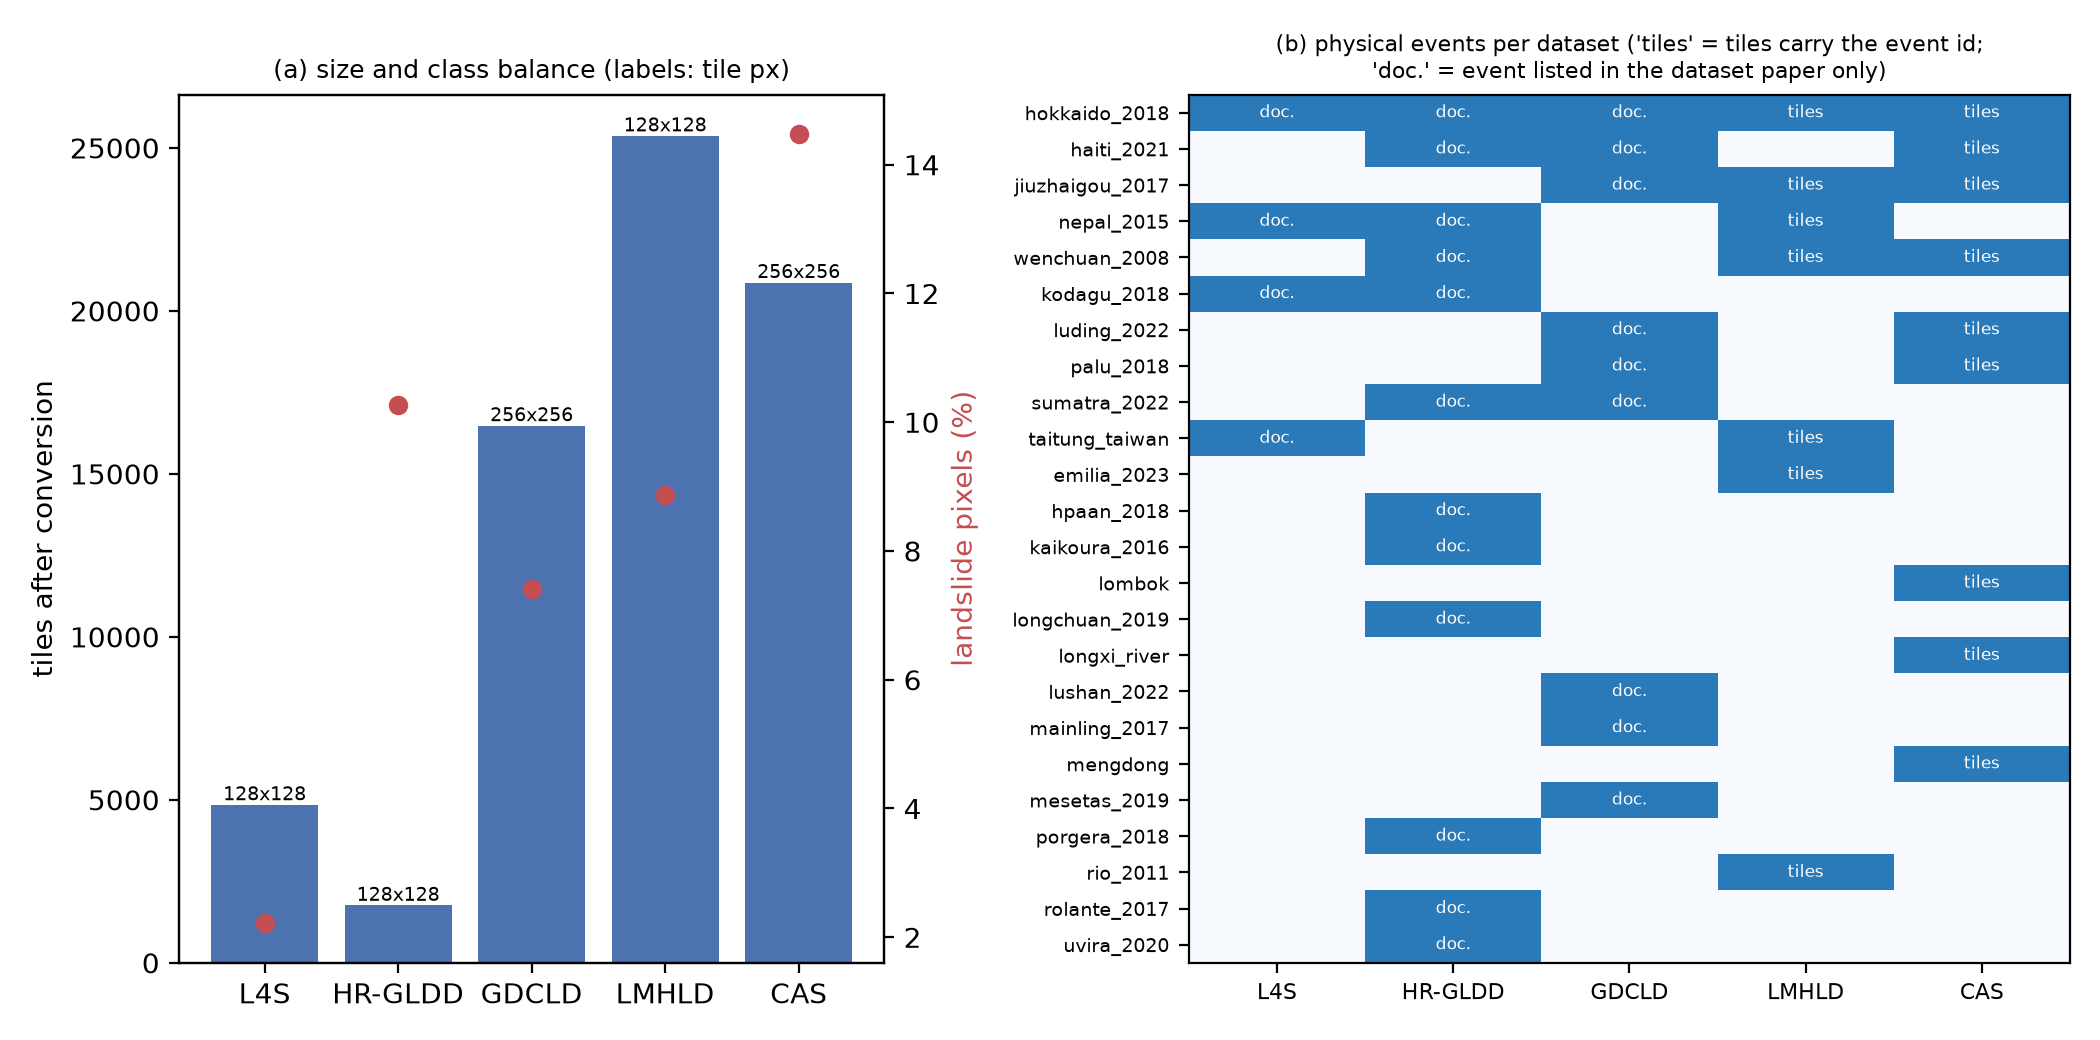
\includegraphics[width=\textwidth]{../figures/fig_data_overview.png}
\caption{(a) Tiles and landslide-pixel share per dataset (labels: tile size in pixels). (b) Documented physical events per dataset. ``tiles'': tiles carry the event identifier; ``doc.'': the event is listed in the dataset paper only. Event membership is partly inferred (Section~\ref{sec:data}).}\label{fig:data}
\end{figure*}

\subsection{Protocols}
\textbf{Protocol A (in-dataset)} uses the official split. LMHLD's official split is a random tile split inside each event, so all its events appear in both train and test; protocol A numbers for LMHLD are therefore not event-isolated. For GDCLD the dataset paper describes training and validation tiles drawn from five events at a 3:1 ratio and test images from four different events~\cite{fang2024gdcld}, so, according to that description, the GDCLD test split is event-isolated from its training data while its validation split shares events with it (we cannot verify this ourselves because its training and validation tiles carry no event identifier). \textbf{Protocol B (leave-one-dataset-out)} tests on every tile of the held-out dataset and trains and validates on the official train and validation tiles of the other four. \textbf{Protocol B-strict} additionally removes every training tile whose documented event also occurs in the held-out dataset (per tile for LMHLD and CAS, which carry event identifiers; the whole dataset for datasets without them). B-strict therefore trains on \TrainStrictMin{} to \TrainStrictMax{} tiles instead of \TrainPlainMin{} to \TrainPlainMax{} for protocol B. \textbf{An important consequence (Table~\ref{tab:composition}):} because Hokkaido 2018 is present in all five datasets and Landslide4Sense, HR-GLDD and GDCLD carry no tile-level event identifier, B-strict drops those three datasets entirely in every fold, so \emph{its training tiles come only from LMHLD and CAS}. B-strict is therefore a transfer from two source datasets with high-resolution RGB/NIR imagery, and differs from protocol B in the sources of its training data as well as in event overlap; Section~\ref{sec:overlap} addresses this confound with a composition-matched control. \textbf{Protocol C} (leave-one-event/region-out inside LMHLD and CAS) was defined and its splits checked for leakage, but was not run (Section~\ref{sec:limits}).

\begin{table}[!t]\centering
\caption{Source datasets of the training tiles in each fold. Under B-strict only LMHLD and CAS contribute.}\label{tab:composition}
\footnotesize
\fitbox{\columnwidth}{\begin{tabular}{llrrrrr}
\toprule
Protocol & Held-out & \multicolumn{5}{c}{Training tiles from source dataset} \\
 & & L4S & HR-GLDD & GDCLD & LMHLD & CAS \\
\midrule
B & L4S & -- & 1{,}119 & 11{,}162 & 17{,}753 & 14{,}687 \\
B & HR-GLDD & 3{,}799 & -- & 11{,}162 & 17{,}753 & 14{,}687 \\
B & GDCLD & 3{,}799 & 1{,}119 & -- & 17{,}753 & 14{,}687 \\
B & LMHLD & 3{,}799 & 1{,}119 & 11{,}162 & -- & 14{,}687 \\
B & CAS & 3{,}799 & 1{,}119 & 11{,}162 & 17{,}753 & -- \\
\midrule
B-strict & L4S & -- & -- & -- & 8{,}363 & 13{,}203 \\
B-strict & HR-GLDD & -- & -- & -- & 11{,}811 & 13{,}203 \\
B-strict & GDCLD & -- & -- & -- & 14{,}500 & 4{,}709 \\
B-strict & LMHLD & -- & -- & -- & -- & 5{,}526 \\
B-strict & CAS & -- & -- & -- & 12{,}678 & -- \\
\bottomrule
\end{tabular}
}
\end{table}

An automated report checks, for every fold, overlapping tile references, groups straddling train and test, byte-identical tiles across train and test, and documented events shared between train and test. All are zero for B, B-strict and C. Protocol A contains one byte-identical near-black no-data crop in GDCLD. Byte hashing cannot detect overlapping neighbouring tiles; this is controlled only by splitting at event or region level.

\subsection{Data issues found while converting}\label{sec:dataissues}
\begin{itemize}\setlength\itemsep{0pt}
\item \textbf{HR-GLDD band order.} The paper describes the bands as red, green, blue and near-infrared~\cite{meena2023hrgldd}, but the arrays appear to be in B,G,R,NIR order. The channel statistics are suggestive but weak (Appendix~\ref{app:channels}): the ordering of channel means matches one of two LMHLD PlanetScope scenes of documented order and not the other. The decisive evidence is behavioural: with the original mapping the held-out HR-GLDD fold reached a landslide \iou{} of \OldOrderSegIouHrgZ{} (SegFormer-B0, seed 0; U-Net \OldOrderUnetIouHrgZ{}) and with the B,G,R,NIR mapping \SegIouHrgZ{} (U-Net \UnetIouHrgZ{}). We tested only these two orderings, and the mapping was changed after the failure on that fold had been observed (Section~\ref{sec:design}). The order is therefore ``very likely'' B,G,R,NIR but not documented by the source.
\item \textbf{LMHLD} is four-band (blue, green, red, near-infrared), not RGB~\cite{liu2025lmhld}; its Rio de Janeiro arrays carry a fifth channel that the paper does not explain, which we drop (assuming red edge).
\item \textbf{CAS} documents more images in its README than are shipped in the archive (\TilesCas{} in our data); several archives are the same site imaged by different sensors, so we group by physical region.
\item The Landslide4Sense Zenodo release includes masks for the test split, which the competition README describes as withheld. The ``MS2LandsNet'' data source cited by~\cite{srivats2026} is a re-upload of Landslide4Sense; MS2LandsNet is a network~\cite{lu2024ms2}.
\end{itemize}

\section{Methods}
\subsection{Models and training}
We use ResNet34-encoder U-Net~\cite{ronneberger2015unet} and DeepLabV3+~\cite{chen2018deeplab} and the MiT-B0 SegFormer~\cite{xie2021segformer} (\SegParamsM{}\,M parameters) from the \url{segmentation_models_pytorch} library~\cite{iakubovskii2019smp}, with ImageNet-pretrained encoders. Cross-dataset runs use RGB (the only input all datasets provide), random \XdCrop\,px crops at native scale (so that 128\,px and 256\,px datasets mix without rescaling), flips and 90$^\circ$ rotations, \XdEpochs{} epochs, batch size \XdBatch{}, AdamW, cosine learning-rate decay, mixed precision and a loss of cross-entropy plus soft Dice (all settings: Appendix Table~\ref{tab:hparams}). The weights of the epoch with the best validation landslide \iou{} are used once on the test set. In cross-dataset runs the per-epoch validation set is a random subset of at most \XdMaxVal{} tiles of the training datasets' validation splits; test data are never subsampled. In-dataset L4S models read all 14 native bands. No per-dataset hyper-parameter tuning was done; the settings were fixed in advance for each protocol family, apart from the two decisions disclosed in Section~\ref{sec:design}.

\subsection{Band adapter}
To let one network accept different sensors, a $1\times1$ convolution maps an 11-slot channel bank (R, G, B, NIR, red edge, SWIR1, SWIR2, slope, DEM, VV, VH) to three channels in front of a pretrained RGB network. It is initialised as the identity on R, G, B and zero elsewhere, so training starts exactly at the RGB model. Slots missing in a dataset are masked, and during training the non-RGB slots are randomly dropped (per sample with probability 0.3, per slot 0.2) so the network does not depend on bands that a target sensor lacks. Landslide4Sense fills 9 of the 11 slots.

\subsection{LoRA teacher and distillation}
A SegFormer-B3 teacher is adapted with LoRA~\cite{hu2022lora} (rank \KdRank{} on the attention and MLP projections of the frozen encoder; \TeachTrainableM{}\,M of \TeachParamsM{}\,M parameters, \TeachTrainPct\%, are trained, including the decoder) for \KdTeacherEpochs{} epochs in each fold. It is then frozen, and the SegFormer-B0 student minimises $(1-\alpha)\,(\mathrm{CE}+\mathrm{Dice}) + \alpha T^2 \mathrm{KL}(p_T^{\mathrm{teacher}}\,\|\,p_T^{\mathrm{student}})$ with $\alpha=\KdAlpha{}$ and $T=\KdTemp{}$~\cite{hinton2015distill}. Neither $\alpha$, $T$ nor the LoRA rank was tuned.

\subsection{Metrics and statistics}
We report landslide \iou{}, mIoU (mean of landslide and background \iou{}), F1 (landslide class), precision and recall at probability threshold 0.5, PR-AUC (histogram estimate over 2{,}000 probability bins) and the expected calibration error (ECE) of the winning class with 15 confidence bins~\cite{guo2017calib}, all accumulated over every test pixel of a held-out dataset. Means are unweighted over datasets. ``Mean $\pm$ std'' is the mean and sample standard deviation over seeds; the five-dataset mean is computed per seed and then summarised. With \NumSeeds{} seeds a standard deviation is itself very uncertain, and with five folds the smallest possible two-sided Wilcoxon $p$ is 0.0625, so we report differences and sign counts and make no significance claims.

\subsection{Efficiency measurement}
Latency was measured on a laptop CPU (Intel Core i5-1135G7, 4 threads, batch 1, fp32, median of at least \LatRuns{} runs after 5 warm-ups, random weights, \url{torch.inference_mode}). GFLOPs count multiply-adds with \url{torch.utils.flop_counter}. These are laptop-CPU figures and not measurements on an embedded accelerator.

\subsection{Evidence conventions and integrity measures}
Four kinds of statements appear below: (E1) values we measured, each generated from a stored result file; (E2) values quoted from other papers, labelled as such and read through a page-retrieval tool rather than from original tables, listed in one file with their source; (E3) values derived by us from E1 or E2; and (E4) interpretations or hypotheses, which we mark with ``we interpret'', ``may'' or ``untested''. Every number in the text and tables is produced by scripts from the run files, and unit tests cover the metrics, splits, band adapter and LoRA implementation. Training was run on a single Tesla T4 per job; GPU non-determinism means runs are not bit-reproducible, and the version of the segmentation library on the GPU runs was not recorded.

\section{Experimental design and disclosures}\label{sec:design}
Each cross-dataset configuration was run with seeds 0, 1 and 2, except the distilled student (seed 0 on all folds, a second seed on two folds), the plain-B and size-matched controls and the teacher (seed 0); the composition-matched control has seeds 0, 1 and 2. In-dataset baselines are single-seed. Two decisions were informed by test results, and we disclose them: (1) after observing the failure on the held-out HR-GLDD fold we examined the channel order and changed the mapping (Section~\ref{sec:dataissues}); (2) we trained SegFormer-B0 on GDCLD for 60 instead of \IndEpochsGdc{} epochs to check for under-training, compared the test results, and kept \IndEpochsGdc{} epochs, which were also not worse on test. Otherwise no model was selected using test data.

\section{Results}
\subsection{In-dataset baselines}\label{sec:inds}
Table~\ref{tab:inds} gives protocol A results (single seed). On Landslide4Sense with all 14 bands the U-Net reaches a landslide \iou{} of \InLfsFourteenUnetIou{} and SegFormer-B0 \InLfsFourteenSegIou{}; restricted to RGB they fall to \InLfsRgbUnetIou{} and \InLfsRgbSegIou{}, and the band adapter on 9 of 11 slots gives \InLfsBankAdpIou{}. On GDCLD, SegFormer-B0 is best (mIoU \InGdcRgbSegMiou{}, \iou{} \InGdcRgbSegIou{}; U-Net \InGdcRgbUnetIou{}) with \ParSeg{}\,M parameters and \GflSegPxTwoFiveSix{} GFLOPs at 256\,px, against \ParUnet{}\,M and \GflUnetPxTwoFiveSix{} for the U-Net; training SegFormer-B0 for 60 epochs did not help on test (\InGdcRgbSixtySegIou{}).

\begin{table*}[!t]\centering
\caption{In-dataset results (protocol A, official test sets, single seed). Landslide4Sense test masks are those shipped in the Zenodo release. All numbers measured by us.}\label{tab:inds}
\footnotesize
\fitbox{\textwidth}{\begin{tabular}{llllrrrrrrrr}
\toprule
Dataset & Input & Model & Params (M) & GFLOPs & mIoU & IoU & F1 & Prec. & Rec. & PR-AUC & ECE \\
\midrule
L4S & 14 bands & U-Net R34 & 24.5 & 2.1 & 73.3 & 48.0 & 64.9 & 62.9 & 67.1 & 0.673 & 0.010 \\
L4S & 14 bands & DeepLabV3+ R34 & 22.5 & 2.1 & 71.9 & 45.3 & 62.3 & 58.3 & 66.9 & 0.636 & 0.011 \\
L4S & 14 bands & SegFormer-B0 & 3.7 & 0.4 & 72.6 & 46.7 & 63.7 & 57.3 & 71.6 & 0.657 & 0.010 \\
L4S & RGB & U-Net R34 & 24.4 & 2.0 & 68.2 & 37.9 & 54.9 & 71.7 & 44.5 & 0.572 & 0.011 \\
L4S & RGB & SegFormer-B0 & 3.7 & 0.4 & 68.8 & 39.2 & 56.3 & 63.1 & 50.8 & 0.556 & 0.011 \\
L4S & bank (9 of 11 slots) & SegFormer-B0 + adapter & 3.7 & 0.4 & 70.2 & 42.2 & 59.4 & 51.5 & 70.2 & 0.604 & 0.011 \\
GDCLD & RGB & U-Net R34 & 24.4 & 7.8 & 69.0 & 38.7 & 55.8 & 68.5 & 47.1 & 0.604 & 0.005 \\
GDCLD & RGB & DeepLabV3+ R34 & 22.4 & 7.9 & 67.0 & 34.8 & 51.7 & 63.2 & 43.7 & 0.562 & 0.005 \\
GDCLD & RGB & SegFormer-B0 & 3.7 & 1.7 & 70.1 & 40.9 & 58.1 & 72.6 & 48.4 & 0.654 & 0.004 \\
GDCLD & RGB & SegFormer-B0, 60 epochs & 3.7 & 1.7 & 69.6 & 40.0 & 57.1 & 61.2 & 53.6 & 0.529 & 0.005 \\
\bottomrule
\end{tabular}
}
\end{table*}

\paragraph{Context from the literature (E2).} Table~\ref{tab:lit} lists values reported by others. On Landslide4Sense the cited papers report U-Net mIoU/F1 of \LitPrithviSevenUNetMiou{}/\LitPrithviSevenUNetFone{}~\cite{szwarcman2024prithvi} and \LitLiUNetMiou{}/\LitLiUNetFone{}~\cite{li2025prithvi}; our U-Net reaches \InLfsFourteenUnetMiou{}/\InLfsFourteenUnetFone{}. We do not read this as an improvement: the inputs (all 14 bands against six bands in \cite{szwarcman2024prithvi}), encoder, loss and checkpoint selection differ, and we did not re-run their pipelines.

For GDCLD our SegFormer-B0 reaches a test mIoU of \InGdcRgbSegMiou{}. The GDCLD paper reports for SegFormer a mIoU of \LitEssdValSegformerMiou{} on its \emph{validation} set but \LitEssdTestSegformerMiou{} on its independent \emph{test} set of four events~\cite{fang2024gdcld}; our figure is \GdcOursMinusEssdTestMiou{} points from the latter. That paper does not state how mIoU or F1 are averaged over classes. Under the assumption that its F1 is a two-class average, the corresponding quantity for our model, derived from our stored \iou{} values, is \InGdcRgbSegMacroFone{} against their \LitEssdTestSegformerFOne{} (our landslide-class F1 alone is \InGdcRgbSegFone{}); we cannot confirm their averaging, input size or model variant, and our model is smaller, trained for fewer epochs, and evaluated on 256\,px downscaled crops. We therefore regard our GDCLD result as broadly consistent with the cited test result; comparing it with the cited \emph{validation} figure would mix splits that differ by \LitEssdValTestGap{} points in that paper alone.

\begin{table*}[!t]\centering
\caption{Values reported by other papers, shown as context only (E2). Read through a page-retrieval tool; table images were not inspected, so every value must be checked against the original. Inputs, splits, models and metric definitions differ from ours.}\label{tab:lit}
\footnotesize
\fitbox{\textwidth}{\begin{tabular}{llllrr}
\toprule
Source & Dataset / split & Model & Input & mIoU & F1 \\
\midrule
\cite{li2025prithvi} & L4S test & U-Net & see source & 70.44 & 59.66 \\
\cite{li2025prithvi} & L4S test & SegFormer & see source & 69.89 & 59.12 \\
\cite{li2025prithvi} & L4S test & Prithvi-EO-2.0-300M & see source & 71.30 & 60.70 \\
\cite{szwarcman2024prithvi} & L4S test & U-Net (ResNet50) & 6 bands & 70.4 & 59.7 \\
\cite{fang2024gdcld} & GDCLD validation & SegFormer & RGB 1024 px & 85.06 & 91.52 \\
\cite{fang2024gdcld} & GDCLD validation & U-Net & RGB 1024 px & 71.07 & 79.54 \\
\cite{fang2024gdcld} & GDCLD test (4 events) & SegFormer & RGB 1024 px & 72.84 & 81.88 \\
\bottomrule
\end{tabular}
}
\end{table*}

\paragraph{Validation overstates test.} In our GDCLD runs the best validation landslide \iou{} exceeds the test \iou{} by \GdcValTestSegGap{} points (SegFormer-B0; \GdcValTestUnetGap{} for the U-Net). The cited GDCLD paper shows a similar pattern in its own numbers (\LitEssdValTestGap{} mIoU points between validation and test). Both are consistent with validation tiles sharing events with training tiles, which is how the dataset paper describes its random 3:1 split within five events, whereas the test images come from four other events~\cite{fang2024gdcld}; we cannot verify the split ourselves, because GDCLD's training and validation tiles carry no event identifier. The test crops also contain a much smaller share of landslide pixels than the training and validation tiles, which lowers \iou{} for the same per-pixel error.

\subsection{Cross-dataset transfer under B-strict}\label{sec:strict}
Table~\ref{tab:strict} and Fig.~\ref{fig:strict} report landslide \iou{} on each held-out dataset (mean $\pm$ std over \NumSeeds{} seeds). SegFormer-B0 reaches \SegIouAllP{} averaged over the five datasets and the U-Net \UnetIouAllP{}. SegFormer-B0 is ahead on \DiffSegUnetPos{} of \DiffSegUnetCnt{} datasets (differences of seed means: HR-GLDD \DiffSegUnetHrg{}, GDCLD \DiffSegUnetGdc{}, LMHLD \DiffSegUnetLmh{}, CAS \DiffSegUnetCas{}; mean \DiffSegUnetMean{}) and behind on Landslide4Sense (\DiffSegUnetLfs{}), where both models vary strongly between seeds (std \SegIouLfsS{} and \UnetIouLfsS{}). The gap on CAS is the largest: the U-Net gets \UnetIouCasP{} against \SegIouCasP{}. Seed 0 of SegFormer-B0 reached \SegIouLfsZ{} on Landslide4Sense whereas the three-seed mean is \SegIouLfsM{}; a single-seed ranking on that fold would have been misleading. Per-seed values are in Appendix Table~\ref{tab:perseed} and further metrics in Appendix Tables~\ref{tab:f1} and~\ref{tab:ece}. We interpret the difference between the two architectures as suggestive evidence for SegFormer-B0 on average, not as a significant effect.

\begin{table*}[!t]\centering
\caption{Landslide \iou{} (\%) on the held-out dataset under B-strict, mean $\pm$ sample std over seeds. $^\dagger$ single seed; $^\ddagger$ two seeds. The last column is the mean over the five datasets, computed per seed. The distilled student has a complete five-dataset set only for seed 0.}\label{tab:strict}
\footnotesize
\fitbox{\textwidth}{\begin{tabular}{lcccccc}
\toprule
Method & L4S & HR-GLDD & GDCLD & LMHLD & CAS & Mean \\
\midrule
U-Net (ResNet34) & 17.8$\pm$6.2 & 30.4$\pm$2.5 & 17.8$\pm$2.6 & 17.5$\pm$1.8 & 3.9$\pm$2.1 & 17.5$\pm$2.9 \\
SegFormer-B0 & 13.4$\pm$9.4 & 36.9$\pm$0.6 & 28.5$\pm$0.2 & 21.8$\pm$6.2 & 21.2$\pm$2.1 & 24.4$\pm$2.9 \\
SegFormer-B0 + band adapter & 13.0$\pm$5.7 & 39.4$\pm$1.7 & 29.6$\pm$0.8 & 19.3$\pm$3.2 & 17.8$\pm$2.5 & 23.8$\pm$1.8 \\
SegFormer-B0 distilled student & 9.6$\pm$0.8$^\ddagger$ & 33.8$^\dagger$ & 27.4$^\dagger$ & 30.1$^\dagger$ & 15.1$\pm$2.8$^\ddagger$ & 22.9$^\dagger$ \\
\bottomrule
\end{tabular}
}
\end{table*}

\begin{figure*}[!t]\centering
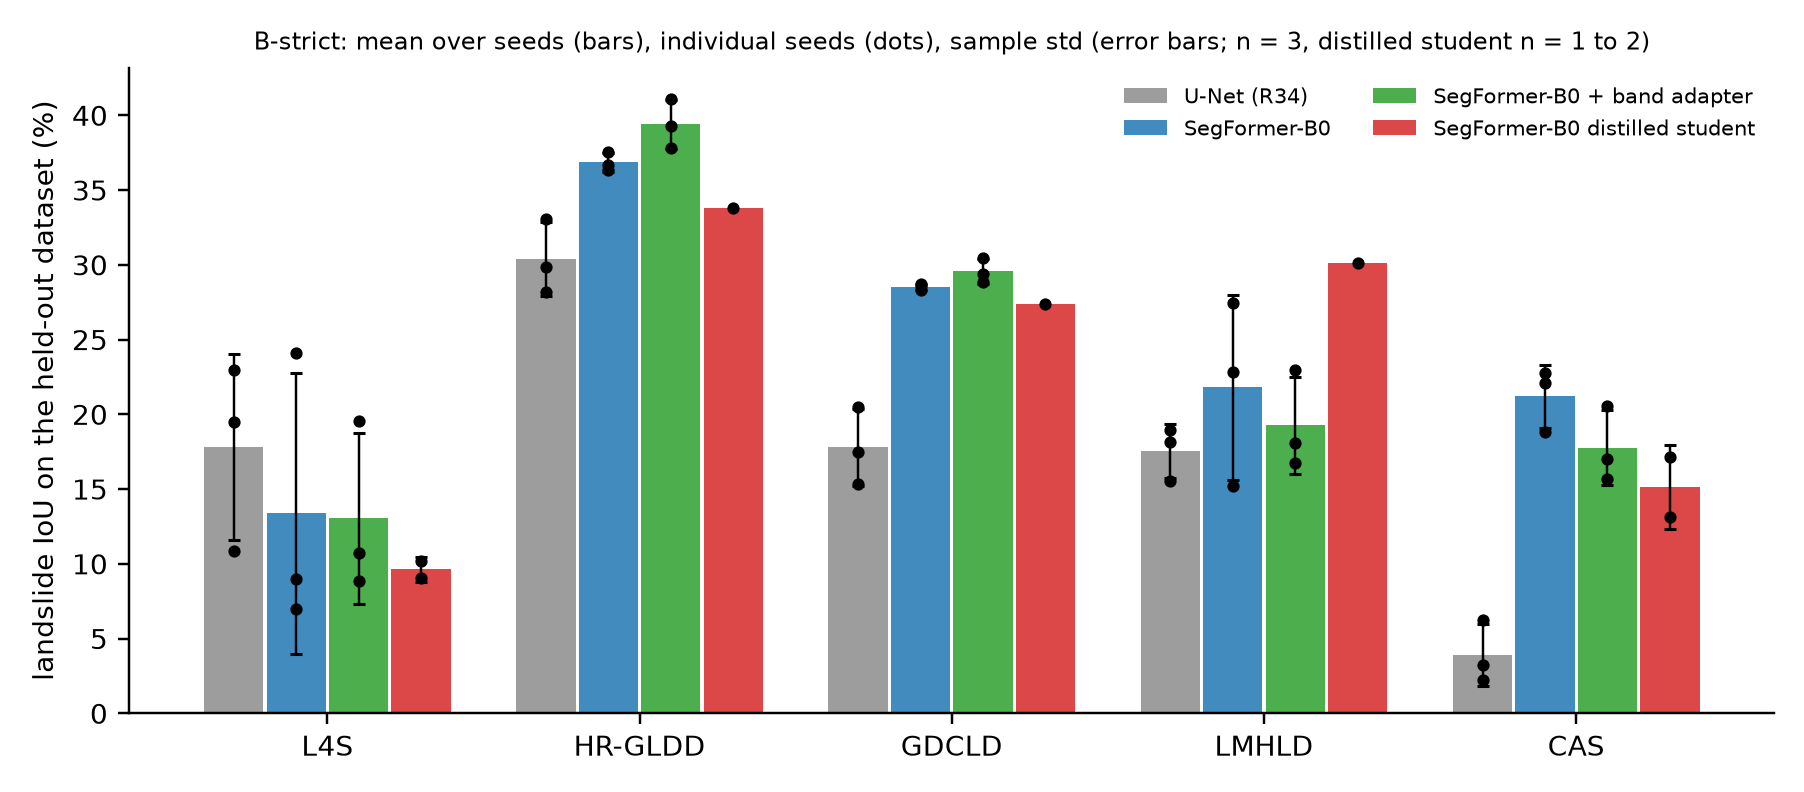
\includegraphics[width=\textwidth]{../figures/fig_strict_bars.png}
\caption{B-strict landslide \iou{} per held-out dataset: means (bars), individual seeds (dots) and sample standard deviation (error bars).}\label{fig:strict}
\end{figure*}

\subsection{Effect of event overlap}\label{sec:overlap}
Protocols B and B-strict differ in three ways at once: the number of training tiles, which source datasets supply them (Table~\ref{tab:composition}), and whether tiles that share events with the held-out dataset are present. We separate these with two SegFormer-B0 controls (Table~\ref{tab:overlap}, Fig.~\ref{fig:overlap}). A \emph{size-matched} control cuts plain B to the B-strict number of tiles, drawn from all four other datasets (seed 0). A \emph{composition-matched} control trains on the same source datasets as B-strict (LMHLD and CAS, excluding the held-out one) and the same number of tiles but does \emph{not} remove event-sharing tiles (\NumSeeds{} seeds); it differs from B-strict only in event overlap.

\paragraph{Total drop and training-set size.} Plain B gives (seed 0) \PlainIouCasZ{} on CAS and \PlainIouGdcZ{} on GDCLD against \SegIouCasZ{} and \SegIouGdcZ{} under B-strict, drops of \OvlTotalCas{} and \OvlTotalGdc{} points; on L4S and LMHLD the drops are \OvlTotalLfs{} and \OvlTotalLmh{} points. Cutting plain B to the B-strict size accounts for only \OvlDataCas{} to \OvlDataGdc{} points of these drops.

\paragraph{Event overlap with the sources held fixed.} Between the composition-matched control and B-strict (Table~\ref{tab:overlap_seeds}), removing event-sharing tiles lowers \iou{} on GDCLD from \CompIouGdcP{} to \SegIouGdcP{} (a difference of \OvlEventsSeedsAbsGdc{} points, far larger than the seed standard deviations) and on CAS from \CompIouCasP{} to \SegIouCasP{} (\OvlEventsSeedsAbsCas{} points, about three times the seed standard deviations). On Landslide4Sense (\OvlEventsSeedsLfs{}) and HR-GLDD (\OvlEventsSeedsHrg{}) the differences are within the seed noise. On LMHLD the composition-matched model scores \emph{lower} than B-strict (\OvlEventsSeedsLmh{}; seed standard deviations \CompIouLmhS{} and \SegIouLmhS{}), a reversal of the size of the noise. Averaged over datasets, keeping events gives \CompIouAllP{} against \SegIouAllP{} (a difference of \OvlEventsSeedsMean{}, higher with events kept on \OvlEventsSeedsPos{} of 5 datasets), a gain dominated by GDCLD.

\paragraph{What remains unseparated.} For CAS most of the plain-B-to-B-strict drop is not the event removal above but the loss of the other source datasets: in seed 0 the composition-matched run is \OvlSourceCas{} points below the size-matched run. Those datasets include data that share events with CAS (for example GDCLD shares Jiuzhaigou, Luding and Hokkaido with it) as well as different sensors and regions, so event overlap and source diversity cannot be separated in that step; the composition-matched comparison isolates only the event overlap \emph{within} the two remaining sources. The plain-B and size-matched runs are single seeds, and the plain-B HR-GLDD fold was made with the wrong channel order and is not reported.

\begin{table*}[!t]\centering
\caption{Event-overlap controls for SegFormer-B0, landslide \iou{} (\%). Plain B and size-matched: seed 0. Composition-matched and B-strict: mean $\pm$ sample std over seeds. These two train on the same source datasets (LMHLD and CAS) and the same number of tiles and differ only in whether event-sharing tiles are present.}\label{tab:overlap}
\footnotesize
\fitbox{\textwidth}{\begin{tabular}{lccccc}
\toprule
Held-out & Plain B & Plain B, size-matched & B-strict & \multicolumn{2}{c}{Difference attributable to} \\
 & (seed 0) & (seed 0) & (seed 0) & training-set size & shared events \\
\midrule
L4S & 27.3 & 22.8 & 24.1 & 4.5 & $-$1.3 \\
HR-GLDD & n/a & 38.1 & 36.7 & n/a & 1.4 \\
GDCLD & 45.3 & 38.9 & 28.6 & 6.4 & 10.3 \\
LMHLD & 24.9 & 19.4 & 22.8 & 5.5 & $-$3.4 \\
CAS & 48.3 & 46.7 & 22.1 & 1.6 & 24.6 \\
\bottomrule
\end{tabular}
}
\end{table*}

\begin{table*}[!t]\centering
\caption{Effect of removing event-sharing tiles with the training sources and size held fixed: difference of seed means (composition-matched minus B-strict; positive means higher with events kept) and the seed standard deviations of the two conditions.}\label{tab:overlap_seeds}
\footnotesize
\fitbox{\textwidth}{\begin{tabular}{lcccc}
\toprule
Held-out & Events kept (composition-matched) & Events removed (B-strict) & Difference of means & Seed std (kept / removed) \\
\midrule
L4S & 14.5 & 13.4 & +1.2 & 7.6 / 9.4 \\
HR-GLDD & 37.7 & 36.9 & +0.8 & 0.7 / 0.6 \\
GDCLD & 45.3 & 28.5 & +16.8 & 0.6 / 0.2 \\
LMHLD & 16.0 & 21.8 & $-$5.8 & 2.9 / 6.2 \\
CAS & 27.7 & 21.2 & +6.5 & 1.7 / 2.1 \\
\midrule
Mean over datasets & 28.3 & 24.4 & +3.9 & 2.3 / 2.9 \\
\bottomrule
\end{tabular}
}
\end{table*}

\begin{figure*}[!t]\centering
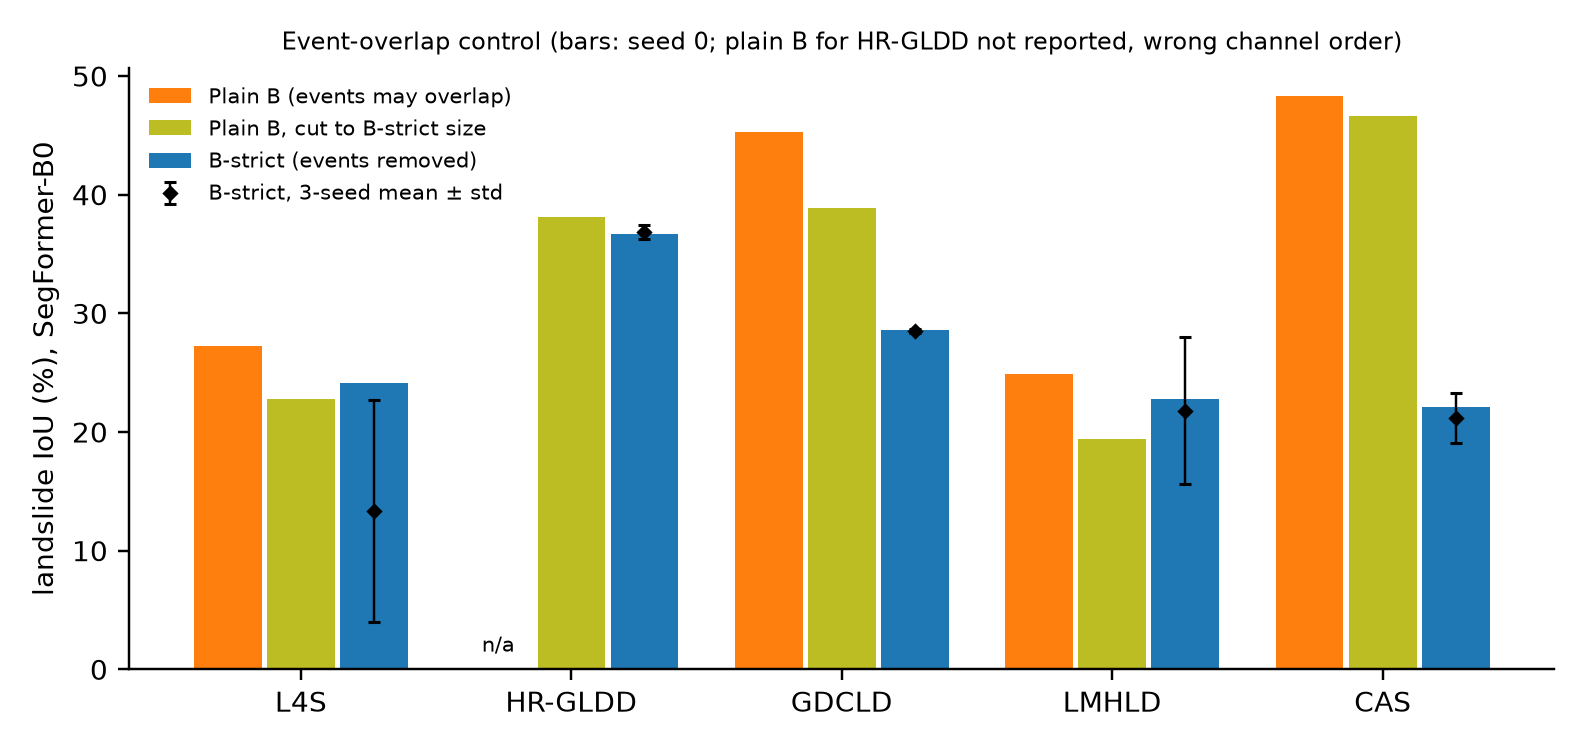
\includegraphics[width=\textwidth]{../figures/fig_overlap.png}
\caption{Event-overlap controls for SegFormer-B0. Bars: seed 0; diamonds with error bars: mean $\pm$ std over three seeds (composition-matched and B-strict).}\label{fig:overlap}
\end{figure*}

\subsection{Band adapter}\label{sec:adapter}
Under B-strict the band adapter gives \AdpIouLfsP{} (L4S), \AdpIouHrgP{} (HR-GLDD), \AdpIouGdcP{} (GDCLD), \AdpIouLmhP{} (LMHLD) and \AdpIouCasP{} (CAS), a five-dataset mean of \AdpIouAllP{} against \SegIouAllP{} for RGB-only SegFormer-B0. Differences of seed means are \DiffAdpSegHrg{} (HR-GLDD), \DiffAdpSegGdc{} (GDCLD), \DiffAdpSegLfs{} (L4S), \DiffAdpSegLmh{} (LMHLD) and \DiffAdpSegCas{} (CAS), positive on \DiffAdpSegPos{} of \DiffAdpSegCnt{} datasets, with a mean of \DiffAdpSegMean{}. There is no detectable cross-dataset benefit in our setting. In-dataset on Landslide4Sense, where the extra bands are present at test time, the adapter does help (\InLfsBankAdpIou{} against \InLfsRgbSegIou{} for RGB only, single seed). The adapter adds essentially no computation (\GflAdpPxOneTwoEight{} against \GflSegPxOneTwoEight{} GFLOPs) and no measurable latency (\LatAdpPxOneTwoEightTFour{} against \LatSegPxOneTwoEightTFour{} ms), and lets one model take RGB, four-band and 14-band inputs. We conjecture, without having tested it, that most training sensors in a B-strict fold provide only RGB, so the extra bands are rarely informative during training.

\subsection{LoRA teacher and distillation}\label{sec:kd}
The SegFormer-B3 teacher (\TeachParamsM{}\,M parameters; \TeachTrainableM{}\,M trained) reaches (seed 0) a mean landslide \iou{} of \TeachIouAllZ{} over the five datasets, \TeachMinusSegZ{} points relative to seed 0 of the RGB SegFormer-B0 (\SegIouAllZ{}); it is \ParamRatioTeachSeg{} times larger and \LatRatioTeachSeg{} times slower on the CPU. The distilled student did not beat the undistilled student (Table~\ref{tab:kd}): its seed-0 five-dataset mean is \KdIouAllZ{} against \SegIouAllZ{}, and it was worse on four of five datasets (differences of seed means: L4S \DiffKdSegLfs{}, HR-GLDD \DiffKdSegHrg{}, GDCLD \DiffKdSegGdc{}, CAS \DiffKdSegCas{}) and better on LMHLD (\DiffKdSegLmh{}, a single seed there). The drops on L4S and CAS reproduced with a second seed (L4S \KdIouLfsP{}, CAS \KdIouCasP{}), so they are not one-off failures, although the undistilled L4S baseline is itself very noisy (\SegIouLfsP{}). This is a negative result for this configuration: we did not tune $\alpha$, $T$ or the LoRA rank, tried one teacher, and did not run rank or distillation-type ablations.

\begin{table*}[!t]\centering
\caption{Teacher and distilled student, B-strict landslide \iou{} (\%). $^\dagger$ single seed; $^\ddagger$ two seeds. The teacher was trained once per fold (seed 0).}\label{tab:kd}
\footnotesize
\fitbox{\textwidth}{\begin{tabular}{lcccc}
\toprule
Held-out & Teacher B3+LoRA (seed 0) & Student, KD & Student, no KD (seed 0) & Student, no KD (mean of seeds) \\
\midrule
L4S & 22.7 & 9.6$\pm$0.8$^\ddagger$ & 24.1 & 13.4$\pm$9.4 \\
HR-GLDD & 38.6 & 33.8$^\dagger$ & 36.7 & 36.9$\pm$0.6 \\
GDCLD & 33.3 & 27.4$^\dagger$ & 28.6 & 28.5$\pm$0.2 \\
LMHLD & 30.1 & 30.1$^\dagger$ & 22.8 & 21.8$\pm$6.2 \\
CAS & 26.3 & 15.1$\pm$2.8$^\ddagger$ & 22.1 & 21.2$\pm$2.1 \\
\midrule
Mean & 30.2 & 22.9$^\dagger$ & 26.9 & 24.4$\pm$2.9 \\
\bottomrule
\end{tabular}
}
\end{table*}

\subsection{Efficiency}\label{sec:eff}
Table~\ref{tab:lat} and Fig.~\ref{fig:pareto} give parameters, GFLOPs and CPU latency. At 128\,px SegFormer-B0 takes \LatSegPxOneTwoEightTFour{} ms with four threads (\ParSeg{}\,M parameters, \GflSegPxOneTwoEight{} GFLOPs, \MbSeg{}\,MB of fp32 weights) against \LatUnetPxOneTwoEightTFour{} ms for the U-Net (\ParUnet{}\,M, \GflUnetPxOneTwoEight{} GFLOPs), a factor of \LatRatioUnetSeg{}, and is on average more accurate under B-strict. Median training time per B-strict fold was \TimeSegMedS{} s for SegFormer-B0 and \TimeUnetMedS{} s for the U-Net on a T4 (a distilled-student fold took \TimeKdMedS{} s plus \TeachMedTrainS{} s for the teacher). Single-thread timings are noisier. On the accuracy axis of Fig.~\ref{fig:pareto}, the adapter and the distilled student sit at the same latency as SegFormer-B0 without an accuracy gain.

\begin{table*}[!t]\centering
\caption{Parameters and CPU latency (median; Intel Core i5-1135G7, batch 1, fp32). The teacher's parameter count is for the base model; with LoRA it is \TeachParamsM{}\,M.}\label{tab:lat}
\footnotesize
\fitbox{\textwidth}{\begin{tabular}{lrrrrrr}
\toprule
Model & Params (M) & Weights fp32 (MB) & GFLOPs, 128 px & 128 px, 1 thread (ms) & 128 px, 4 threads (ms) & 256 px, 4 threads (ms) \\
\midrule
U-Net R34 & 24.4 & 98 & 1.96 & 92 & 45 & 141 \\
DeepLabV3+ R34 & 22.4 & 90 & 1.97 & 90 & 53 & 139 \\
SegFormer-B0 & 3.7 & 15 & 0.42 & 28 & 22 & 78 \\
SegFormer-B0 + band adapter & 3.7 & 15 & 0.43 & 41 & 23 & 88 \\
SegFormer-B3 (teacher) & 44.6 & 178 & 2.26 & 176 & 88 & 289 \\
\bottomrule
\end{tabular}
}
\end{table*}

\begin{figure}[!t]\centering
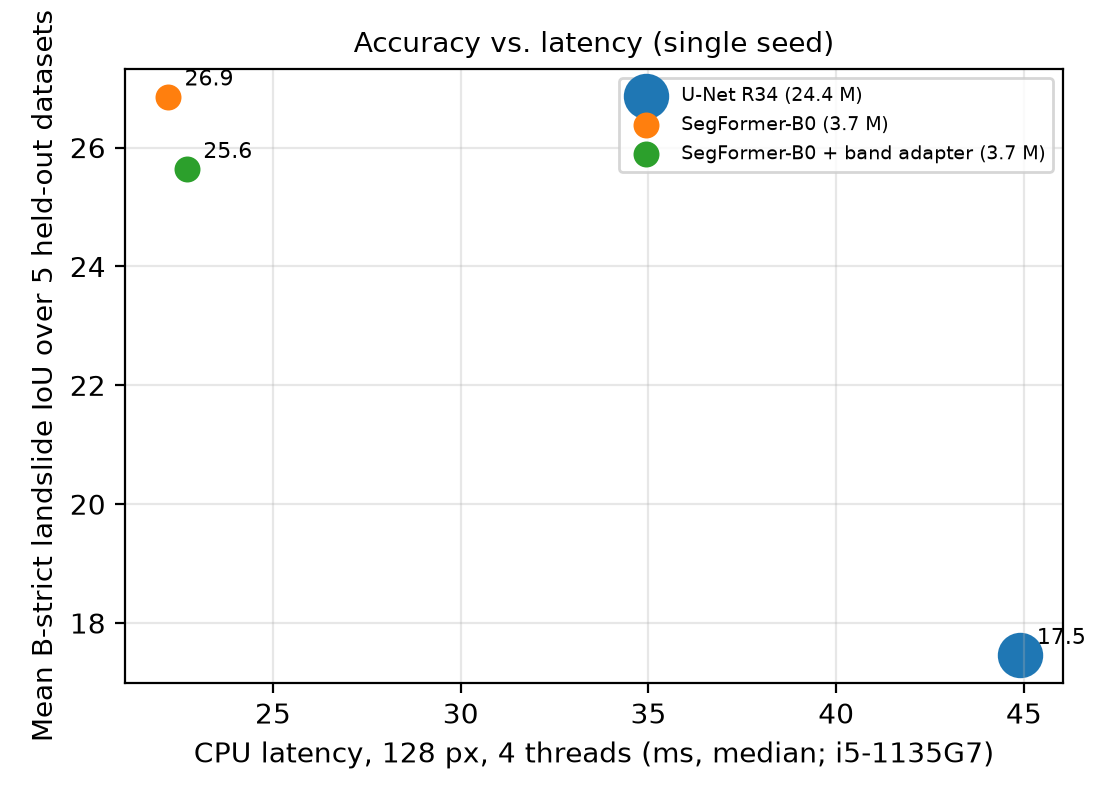
\includegraphics[width=\columnwidth]{../figures/fig_pareto.png}
\caption{Mean B-strict landslide \iou{} against CPU latency (128\,px, 4 threads); error bars are the std over seeds where more than one seed is available (the distilled student has one complete seed).}\label{fig:pareto}
\end{figure}

\subsection{Calibration}\label{sec:calib}
Pixel-level ECE is low in-dataset (\InLfsFourteenUnetEce{} for the L4S U-Net; \InGdcRgbSegEce{} for the GDCLD SegFormer-B0) but higher on unseen datasets: five-dataset means are \SegEceAllP{} for SegFormer-B0 and \UnetEceAllP{} for the U-Net, with the largest values on CAS (\SegEceCasP{} and \UnetEceCasP{}) and, for the U-Net, on LMHLD (\UnetEceLmhP{}). Reliability curves (Fig.~\ref{fig:rel}) lie below the diagonal in almost all panels, so confident predictions are usually right less often than their confidence implies; the exception in the plotted seed is the U-Net on HR-GLDD at mid confidence, where it is under-confident. In the plotted seed the U-Net's confident predictions on LMHLD and CAS are barely better than chance. ECE is computed over all pixels and is dominated by background, which limits its meaning for rare-class segmentation.

\begin{figure*}[!t]\centering
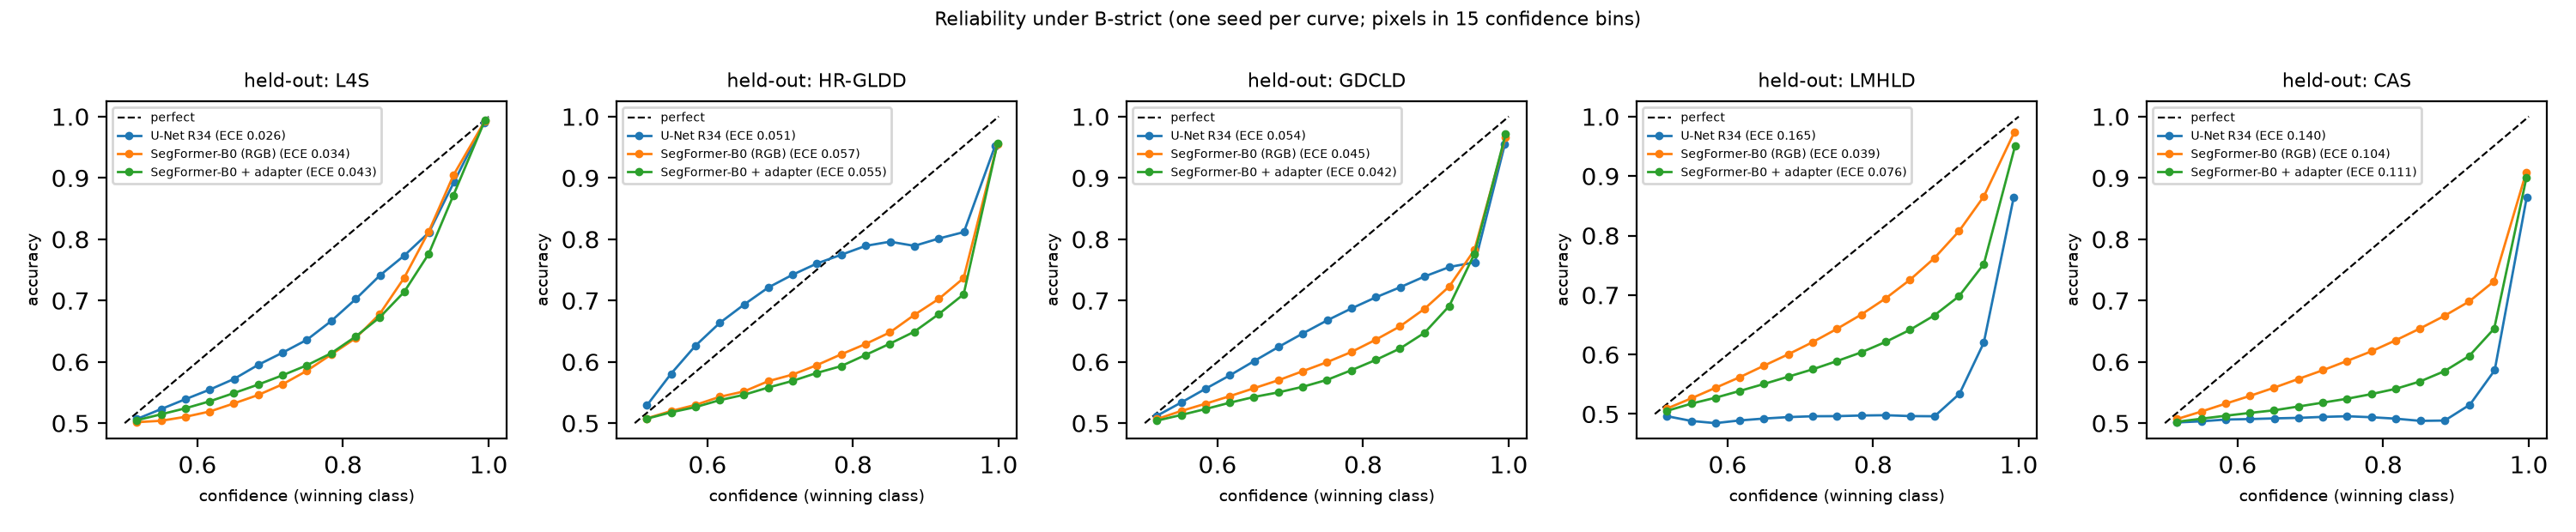
\includegraphics[width=\textwidth]{../figures/fig_reliability.png}
\caption{Reliability diagrams under B-strict (seed 1; 15 confidence bins; accuracy of the winning class).}\label{fig:rel}
\end{figure*}

\subsection{Failure analysis}\label{sec:fail}
Failures are local rather than uniform (Appendix Table~\ref{tab:regions}; size-matched SegFormer-B0 runs, seed 0): on CAS, Palu reaches \RegCasPalu{} and Lombok \RegCasLombok{} against \RegCasJiuzhaivalley{} for Jiuzhai valley; on GDCLD, Mesetas \RegGdcMesetas{} and Lushan \RegGdcLushan{} against \RegGdcPalu{} for Palu; on LMHLD, Wenchuan (IKONOS, 0.8\,m) \RegLmhWenchuanChina{} against \RegLmhRestMin{} to \RegLmhRestMax{} for the other six events. Fig.~\ref{fig:fail} shows the two typical outcomes on held-out CAS (adapter model, seed 1): tiles whose landslides cover \ExWorstMinPct{} to \ExWorstMaxPct\% of the area and are missed entirely (\iou{} \ExWorstIouMax{}), and near-whole-tile landslides in 0.2\,m UAV imagery of Jiuzhai valley that are easy (\iou{} \ExBestIouMin{} to \ExBestIouMax{}). Many tiles tie at \iou{} 0.00 and our export breaks ties by tile index, so the six ``worst'' tiles all come from one region (Hokkaido Iburi-Tobu, a 3\,m satellite subset); they illustrate a failure mode and are not a ranking of the worst cases.

\begin{figure*}[!t]\centering
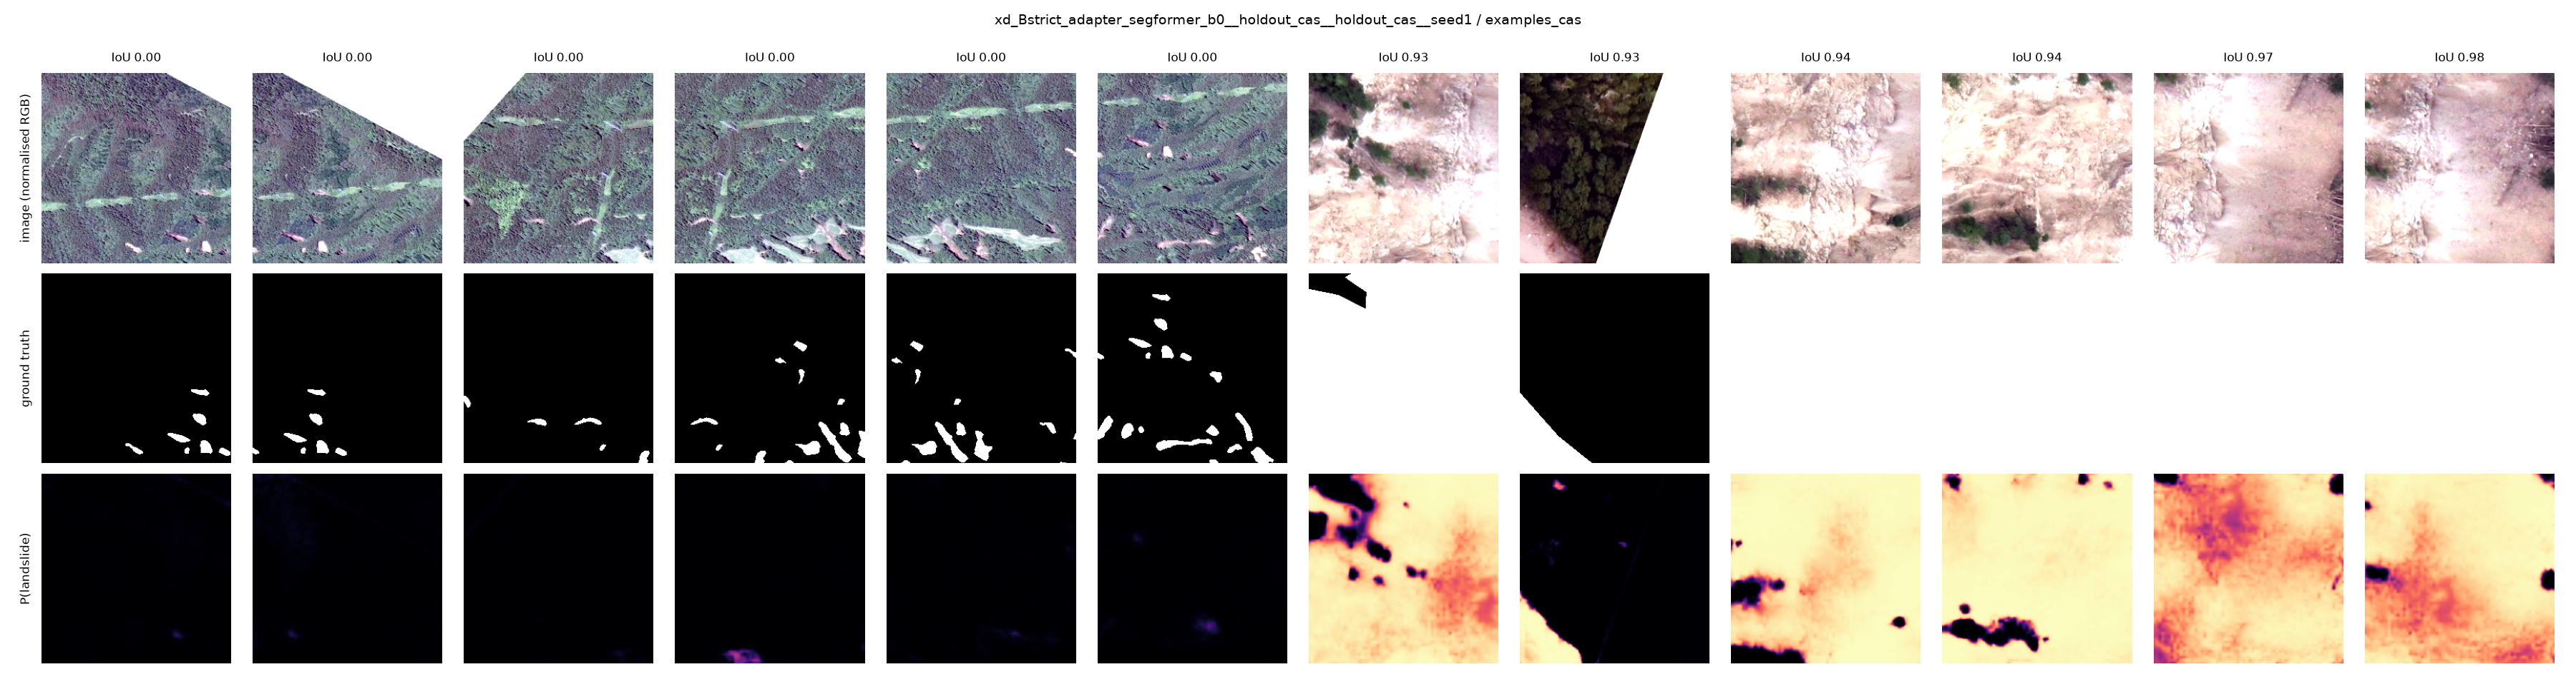
\includegraphics[width=\textwidth]{../figures/fig_failures.png}
\caption{Left six: lowest tile-\iou{} examples; right six: highest, among tiles with at least 1\% landslide pixels (held-out CAS, band-adapter model, seed 1). Rows: normalised RGB, ground truth, predicted landslide probability.}\label{fig:fail}
\end{figure*}

\section{Discussion}
\paragraph{What the evidence supports.} (1) Scores obtained without removing event-sharing training data can substantially overstate cross-dataset performance on some datasets: with the training sources and size held fixed, the effect is large for GDCLD, moderate for CAS and not detectable for the other three (three seeds); beyond that, the larger source pool of plain B contributes its own, partly inseparable, benefit. (2) Under event-isolated transfer a compact SegFormer-B0 is, on average over datasets and seeds, at least as accurate as a ResNet34 U-Net with several times more parameters, at half the CPU latency, although the ranking varies by dataset and the difference is not shown to be significant. (3) Neither the band adapter nor distillation from a larger LoRA teacher improved the compact model in our configuration. (4) With few exceptions, models were over-confident on unseen datasets. (5) A single misdocumented channel order can change a transfer result by an order of magnitude, and several dataset documents are inconsistent with the files.

\paragraph{What it does not support.} We did not show that SegFormer-style models are intrinsically better at transfer: one family was tried, with short training, RGB input and no tuning. We did not show that distillation or band adaptation cannot work: we tested one configuration each. We cannot attribute the validation--test gap on GDCLD to event overlap, because event identifiers are missing for its training and validation tiles. The effect of event overlap is isolated only within the two source datasets that remain under B-strict; for datasets removed wholesale, event overlap and source diversity are confounded. Event membership is partly inferred.

\paragraph{Implications for benchmark design (recommendations, E4).} Report which physical events a test set shares with the training data; prefer a held-out dataset or event over a held-out tile; report several seeds, since a single seed misranked methods on one fold in our data; report calibration and latency, not only overlap metrics; and publish tile-level event or region identifiers with datasets so that isolation can be checked. Event identifiers were available only for two of the five datasets.

\paragraph{Why the adapter and distillation may not have helped (hypotheses, untested).} For the adapter, the lack of sensors with extra bands in the training pool of a B-strict fold; for distillation, a teacher whose own transfer is only moderately better than the student, a short schedule, and untuned $\alpha$ and $T$. These would need dedicated experiments.

\section{Limitations}\label{sec:limits}
\begin{itemize}\setlength\itemsep{0pt}
\item \textbf{Seeds and statistics.} The headline B-strict comparisons use \NumSeeds{} seeds; the teacher, the distilled student, the plain-B and size-matched controls, the per-region analysis and the in-dataset baselines are single- or two-seed. Seed variation is large on some folds, and five folds do not allow a significance test at the 5\% level.
\item \textbf{Untuned architecture comparison.} Learning rate and weight decay differ between the SegFormer and CNN families (Table~\ref{tab:hparams}) and were not tuned for any model, so the U-Net/SegFormer comparison is a comparison of untuned defaults and could change with tuning.
\item \textbf{Scope of models and inputs.} One compact transformer and two CNNs, RGB (or the adapter's bands), \XdCrop\,px crops and \XdEpochs{} epochs; no foundation models (excluded by the compute budget), no longer training, no tuning. GDCLD was downscaled by 4 and CAS by about 2 (from the 512\,px tiles we inspected), losing detail visible at 0.2 to 1\,m resolution in the UAV subsets.
\item \textbf{Protocol.} Event assignments are partly inferred from place names, so residual overlap cannot be excluded; L4S, HR-GLDD and the GDCLD training and validation tiles carry no event identifiers, so those datasets can only be held out whole; protocol C was not run.
\item \textbf{Data.} The HR-GLDD band order and the fifth LMHLD Rio channel are inferred. CAS has no negative tiles, so false-alarm statistics are unavailable. The LMHLD protocol-A split and the GDCLD validation split are not event-isolated.
\item \textbf{Metrics.} ECE is pixel-level and dominated by background; PR-AUC is a histogram estimate; F1 is for the landslide class.
\item \textbf{Hardware.} CPU latency on one laptop; no embedded accelerator, no energy measurement.
\item \textbf{Test-informed decisions.} The HR-GLDD channel mapping and the 60-epoch GDCLD check used test results (Section~\ref{sec:design}).
\item \textbf{Literature.} Several related works are known from abstracts only; quoted external numbers were read via a retrieval tool and must be re-checked against the originals; the novelty statement rests on a limited search.
\item \textbf{Reproducibility.} Runs are not bit-reproducible on GPU, and the library version on the GPU runs was not recorded.
\end{itemize}

\section{Conclusions}
Under an event-isolated leave-one-dataset-out protocol over five public datasets, a compact SegFormer-B0 transferred, on average, at least as well as a larger U-Net at half the CPU latency, but absolute transfer accuracy was low (mean landslide \iou{} \SegIouAllM{}), models were generally over-confident, and neither a band adapter nor distillation from a LoRA teacher helped. With the training sources held fixed, removing event-sharing tiles lowered scores clearly on GDCLD and moderately on CAS, and not detectably on the other three datasets. The main practical message is methodological: report event overlap, use several seeds, and check the documentation of channel order and splits before drawing conclusions. We release the code, splits, leakage report and per-run results so that these checks can be repeated.

\appendices
\section{Additional results}
\begin{table*}[!t]\centering
\caption{B-strict F1 (\%) of the landslide class, mean $\pm$ std over seeds ($^\dagger$ one seed, $^\ddagger$ two).}\label{tab:f1}
\footnotesize
\fitbox{\textwidth}{\begin{tabular}{lcccccc}
\toprule
Method & L4S & HR-GLDD & GDCLD & LMHLD & CAS & Mean \\
\midrule
U-Net (ResNet34) & 29.9$\pm$9.2 & 46.6$\pm$2.9 & 30.2$\pm$3.7 & 29.8$\pm$2.6 & 7.5$\pm$3.8 & 28.8$\pm$4.1 \\
SegFormer-B0 & 22.8$\pm$14.0 & 53.9$\pm$0.7 & 44.4$\pm$0.2 & 35.5$\pm$8.4 & 35.0$\pm$2.9 & 38.3$\pm$4.2 \\
SegFormer-B0 + band adapter & 22.8$\pm$8.7 & 56.5$\pm$1.7 & 45.6$\pm$1.0 & 32.2$\pm$4.5 & 30.1$\pm$3.6 & 37.5$\pm$2.6 \\
SegFormer-B0 distilled student & 17.6$\pm$1.4$^\ddagger$ & 50.5$^\dagger$ & 43.0$^\dagger$ & 46.3$^\dagger$ & 26.2$\pm$4.3$^\ddagger$ & 36.3$^\dagger$ \\
\bottomrule
\end{tabular}
}
\end{table*}
\begin{table*}[!t]\centering
\caption{B-strict expected calibration error (pixel-level, 15 bins), mean $\pm$ std over seeds ($^\dagger$ one seed, $^\ddagger$ two).}\label{tab:ece}
\footnotesize
\fitbox{\textwidth}{\begin{tabular}{lcccccc}
\toprule
Method & L4S & HR-GLDD & GDCLD & LMHLD & CAS & Mean \\
\midrule
U-Net (ResNet34) & 0.016$\pm$0.009 & 0.058$\pm$0.006 & 0.052$\pm$0.003 & 0.168$\pm$0.008 & 0.142$\pm$0.003 & 0.087$\pm$0.003 \\
SegFormer-B0 & 0.026$\pm$0.022 & 0.055$\pm$0.002 & 0.044$\pm$0.001 & 0.044$\pm$0.007 & 0.108$\pm$0.005 & 0.055$\pm$0.006 \\
SegFormer-B0 + band adapter & 0.036$\pm$0.029 & 0.051$\pm$0.003 & 0.041$\pm$0.002 & 0.058$\pm$0.016 & 0.112$\pm$0.002 & 0.060$\pm$0.009 \\
SegFormer-B0 distilled student & 0.034$\pm$0.019$^\ddagger$ & 0.056$^\dagger$ & 0.041$^\dagger$ & 0.027$^\dagger$ & 0.120$\pm$0.001$^\ddagger$ & 0.053$^\dagger$ \\
\bottomrule
\end{tabular}
}
\end{table*}
\begin{table}[!t]\centering
\caption{B-strict landslide \iou{} (\%) per seed.}\label{tab:perseed}
\footnotesize
\fitbox{\columnwidth}{\begin{tabular}{llccc}
\toprule
Method & Held-out & Seed 0 & Seed 1 & Seed 2 \\
\midrule
U-Net (ResNet34) & L4S & 19.5 & 10.9 & 23.0 \\
U-Net (ResNet34) & HR-GLDD & 29.9 & 28.2 & 33.1 \\
U-Net (ResNet34) & GDCLD & 17.5 & 15.4 & 20.5 \\
U-Net (ResNet34) & LMHLD & 18.2 & 15.5 & 19.0 \\
U-Net (ResNet34) & CAS & 2.3 & 3.2 & 6.2 \\
\midrule
SegFormer-B0 & L4S & 24.1 & 9.0 & 7.0 \\
SegFormer-B0 & HR-GLDD & 36.7 & 37.6 & 36.3 \\
SegFormer-B0 & GDCLD & 28.6 & 28.7 & 28.3 \\
SegFormer-B0 & LMHLD & 22.8 & 27.4 & 15.2 \\
SegFormer-B0 & CAS & 22.1 & 22.8 & 18.8 \\
\midrule
SegFormer-B0 + band adapter & L4S & 19.5 & 10.7 & 8.9 \\
SegFormer-B0 + band adapter & HR-GLDD & 41.1 & 39.3 & 37.8 \\
SegFormer-B0 + band adapter & GDCLD & 28.9 & 30.5 & 29.4 \\
SegFormer-B0 + band adapter & LMHLD & 18.1 & 22.9 & 16.8 \\
SegFormer-B0 + band adapter & CAS & 20.6 & 15.7 & 17.0 \\
\midrule
SegFormer-B0 distilled student & L4S & 10.2 & 9.1 & -- \\
SegFormer-B0 distilled student & HR-GLDD & 33.8 & -- & -- \\
SegFormer-B0 distilled student & GDCLD & 27.4 & -- & -- \\
SegFormer-B0 distilled student & LMHLD & 30.1 & -- & -- \\
SegFormer-B0 distilled student & CAS & 13.1 & 17.1 & -- \\
\bottomrule
\end{tabular}
}
\end{table}
\begin{table}[!t]\centering
\caption{Per-region or per-event landslide \iou{} (\%) for SegFormer-B0 under size-matched plain B (seed 0), ascending.}\label{tab:regions}
\footnotesize
{\setlength{\textwidth}{\columnwidth}\fitbox{\columnwidth}{\begin{tabular}{ll}
\toprule
Held-out dataset & Landslide IoU by region/event (ascending) \\
\midrule
CAS & Palu 1.9, Lombok 9.6, Hokkaido Iburi-Tobu 19.6, Tiburon Peninsula 26.2, Wenchuan 26.7, Moxitaidi 37.7, Longxi River 41.8, Moxi town 43.5, Mengdong Township 50.2, Jiuzhai valley 55.5 \\
GDCLD & Mesetas 2.2, Lushan 13.2, Sumarta 31.1, Palu 31.8 \\
LMHLD & Wenchuan China 4.5, Gorkha Nepal 19.1, Taiwan China 19.2, Jiuzhaigou China 21.2, Emilia-Romagna Italy 22.5, Hokkaido Japan 28.3, Rio de Janeiro Brazil 32.7 \\
\bottomrule
\end{tabular}
}}
\end{table}

\section{Event assignment}\label{app:events}
\begin{table}[!t]\centering
\caption{Documented physical events per dataset (T: tiles carry the event identifier; D: listed in the dataset paper only). Source: \texttt{configs/dataset\_events.json}; some assignments are inferred from place names.}\label{tab:events}
\footnotesize
\fitbox{\columnwidth}{\begin{tabular}{lccccc}
\toprule
Event & L4S & HR-GLDD & GDCLD & LMHLD & CAS \\
\midrule
hokkaido\_2018 & D & D & D & T & T \\
haiti\_2021 &  & D & D &  & T \\
jiuzhaigou\_2017 &  &  & D & T & T \\
nepal\_2015 & D & D &  & T &  \\
wenchuan\_2008 &  & D &  & T & T \\
kodagu\_2018 & D & D &  &  &  \\
luding\_2022 &  &  & D &  & T \\
palu\_2018 &  &  & D &  & T \\
sumatra\_2022 &  & D & D &  &  \\
taitung\_taiwan & D &  &  & T &  \\
emilia\_2023 &  &  &  & T &  \\
hpaan\_2018 &  & D &  &  &  \\
kaikoura\_2016 &  & D &  &  &  \\
lombok &  &  &  &  & T \\
longchuan\_2019 &  & D &  &  &  \\
longxi\_river &  &  &  &  & T \\
lushan\_2022 &  &  & D &  &  \\
mainling\_2017 &  &  & D &  &  \\
mengdong &  &  &  &  & T \\
mesetas\_2019 &  &  & D &  &  \\
porgera\_2018 &  & D &  &  &  \\
rio\_2011 &  &  &  & T &  \\
rolante\_2017 &  & D &  &  &  \\
uvira\_2020 &  & D &  &  &  \\
\bottomrule
\end{tabular}
}
\end{table}

\section{Settings}
\begin{table*}[!t]\centering
\caption{Training settings.}\label{tab:hparams}
\footnotesize
\fitbox{\textwidth}{\begin{tabular}{lll}
\toprule
Setting & Cross-dataset runs (B, B-strict) & In-dataset runs (A) \\
\midrule
Epochs & 10 & 50 (L4S), 20 (GDCLD) \\
Batch size & 32 & 32 \\
Input & RGB, random 128 px crops at native scale & native channels (L4S), RGB (GDCLD); full tiles \\
Optimiser & AdamW & AdamW \\
Learning rate / weight decay, SegFormer-B0 & 0.0002 / 0.01 & 0.0002 / 0.01 \\
Learning rate / weight decay, U-Net & 0.0003 / 0.0001 & 0.0003 / 0.0001 \\
Schedule & cosine annealing to zero & cosine annealing to zero \\
Loss & cross-entropy + soft Dice & cross-entropy + soft Dice \\
Augmentation & flips, 90$^\circ$ rotations, random crop & flips, 90$^\circ$ rotations \\
Validation set (checkpoint selection) & $\leq$3{,}000 random tiles of the training datasets' validation splits & official validation split \\
Precision & mixed (fp16 autocast) & mixed (fp16 autocast) \\
Teacher / distillation & \multicolumn{2}{l}{SegFormer-B3, LoRA rank 8 on 140 linear layers, 10 epochs; $\alpha=0.5$, $T=2.0$} \\
\bottomrule
\end{tabular}
}
\end{table*}

\section{HR-GLDD channel statistics}\label{app:channels}
Table~\ref{tab:channels} gives mean channel values of the HR-GLDD arrays and of LMHLD scenes whose order is documented as B,G,R,NIR. For HR-GLDD the ordering of the first three channel means (channel~1 $<$ channel~3 $<$ channel~2) is the one that B,G,R would give in one PlanetScope scene (Hokkaido: B $<$ R $<$ G) but not in the other (Taiwan: B $<$ G $<$ R), and values are on different scales (reflectance fractions against digital numbers). The statistics are therefore weak evidence. The decisive evidence is the transfer result in Section~\ref{sec:dataissues}, which supports the B,G,R,NIR mapping only in the sense that it works much better than R,G,B,NIR; we did not test other permutations.
\begin{table*}[!t]\centering
\caption{Mean channel values (HR-GLDD: reflectance fractions in array order; LMHLD: digital numbers in documented B,G,R,NIR order).}\label{tab:channels}
\footnotesize
\fitbox{\textwidth}{\begin{tabular}{llrrrrl}
\toprule
Scene & Sensor & ch.\ 1 & ch.\ 2 & ch.\ 3 & NIR & Order of first three channels \\
\midrule
HR-GLDD (array order) & PlanetScope & 0.109 & 0.150 & 0.140 & 0.500 & ch.1 $<$ ch.3 $<$ ch.2 \\
LMHLD Taiwan (B,G,R) & PlanetScope & 220 & 404 & 433 & 2220 & B $<$ G $<$ R \\
LMHLD Hokkaido (B,G,R) & PlanetScope & 336 & 412 & 386 & 2484 & B $<$ R $<$ G \\
LMHLD Gorkha (B,G,R) & Sentinel-2 & 862 & 1124 & 1331 & 2081 & B $<$ G $<$ R \\
LMHLD Jiuzhaigou (B,G,R) & Gaofen-2 & 369 & 589 & 568 & 2387 & B $<$ R $<$ G \\
LMHLD Emilia-Romagna (B,G,R) & Sentinel-2 & 1472 & 1705 & 1627 & 4111 & B $<$ R $<$ G \\
LMHLD Wenchuan (B,G,R) & IKONOS & 459 & 1253 & 1063 & 4442 & B $<$ R $<$ G \\
\bottomrule
\end{tabular}
}
\end{table*}

\section{Provenance}
All results in this paper are generated from \NumRunsTotal{} stored run files by \url{scripts/make_paper_assets.py} (numbers, tables, bibliography), \url{scripts/make_figures.py}, \url{scripts/make_figures_paper.py} and \url{scripts/make_fig_data.py} (figures); the table of every macro and its value is \url{paper/generated/numbers_provenance.json}. Runs made with the wrong HR-GLDD channel order were excluded and are kept separately.

\section*{Data and code availability}
Code, splits, the leakage report, per-run result files, tables and figures are in a public repository (\url{https://github.com/Edith-Stark06/landslide-cross-region}). The datasets are available from their original sources and are not redistributed (Landslide4Sense, HR-GLDD, GDCLD, LMHLD and CAS Landslide are on Zenodo: \url{10.5281/zenodo.10463239}, \url{7189381}, \url{13612636}, \url{17258777}, \url{10294997}); CAS is licensed CC BY-NC 4.0, the others CC BY 4.0 according to their Zenodo records. Trained model weights were not saved or released.

\section*{Declarations}
\paragraph{Funding.} \todo{To be completed by the authors.}
\paragraph{Competing interests.} \todo{To be completed by the authors.}
\paragraph{Author contributions (CRediT).} \todo{To be completed by the authors.}
\paragraph{Ethics.} \todo{To be confirmed by the authors. The study uses only public third-party datasets under their licences and no human or animal subjects, as far as we are aware.}
\paragraph{Acknowledgements.} \todo{To be completed by the authors.} Compute: free-tier GPU sessions (Tesla T4) on Kaggle and one laptop CPU.
\paragraph{Use of AI tools.} \todo{To be confirmed by the authors against the target journal's policy.} The analysis code, the figures and the manuscript draft were prepared with the assistance of a generative AI system (Claude, Anthropic). All numbers in the text and tables are generated from stored run files by scripts included in the repository, and the authors remain responsible for the content.

\FloatBarrier
\begin{thebibliography}{99}
\bibitem{srivats2026} R. Srivats, D. R. Johnson, G. Logeswari, R. Saimirra, M. Siddiqui, and A. Sharma, ``A multi-modal deep learning framework with GAN-based fusion for enhanced landslide detection,'' \emph{PLoS ONE}, 2026, doi: 10.1371/journal.pone.0347324.
\bibitem{jiang2026review} P. Jiang, Z. Ma, and G. Mei, ``Review article: deep learning for potential landslide identification: data, models, applications, challenges, and opportunities,'' \emph{Nat. Hazards Earth Syst. Sci.}, vol. 26, pp. 487--529, 2026, doi: 10.5194/nhess-26-487-2026.
\bibitem{ghorbanzadeh2022} O. Ghorbanzadeh et al., ``The outcome of the 2022 Landslide4Sense competition: advanced landslide detection from multisource satellite imagery,'' \emph{IEEE J. Sel. Topics Appl. Earth Obs. Remote Sens.}, vol. 15, pp. 9927--9942, 2022, doi: 10.1109/JSTARS.2022.3220845, Data: doi: 10.5281/zenodo.10463239.
\bibitem{fang2024gdcld} C. Fang, X. Fan, X. Wang, L. Nava, H. Zhong, X. Dong, J. Qi, and F. Catani, ``A globally distributed dataset of coseismic landslide mapping via multi-source high-resolution remote sensing images,'' \emph{Earth Syst. Sci. Data}, vol. 16, pp. 4817--4842, 2024, doi: 10.5194/essd-16-4817-2024.
\bibitem{xu2024cas} Y. Xu, C. Ouyang, Q. Xu, D. Wang, B. Zhao, and Y. Luo, ``CAS Landslide Dataset: a large-scale and multisensor dataset for deep learning-based landslide detection,'' \emph{Sci. Data}, vol. 11, Art. no. 12, 2024, doi: 10.1038/s41597-023-02847-z.
\bibitem{meena2023hrgldd} S. R. Meena, L. Nava, K. Bhuyan, S. Puliero, L. P. Soares, H. C. Dias, M. Floris, and F. Catani, ``HR-GLDD: a globally distributed dataset using generalized deep learning (DL) for rapid landslide mapping on high-resolution (HR) satellite imagery,'' \emph{Earth Syst. Sci. Data}, vol. 15, no. 7, pp. 3283--3298, 2023, doi: 10.5194/essd-15-3283-2023.
\bibitem{liu2025lmhld} G. Liu, Y. Wang, X. Chen, B. Du, P. Li, Y. Wu, and Z. Fang, ``LMHLD: a large-scale multi-source high-resolution landslide dataset for landslide detection based on deep learning,'' arXiv:2502.19866, 2025.
\bibitem{hohn2025sen12} P. H\"ohn, K. Heidler, R. Behling, and X. X. Zhu, ``A spatio-temporal dataset for satellite-based landslide detection,'' \emph{Sci. Data}, vol. 12, Art. no. 1772, 2025, doi: 10.1038/s41597-025-06167-2.
\bibitem{xie2021segformer} E. Xie, W. Wang, Z. Yu, A. Anandkumar, J. M. Alvarez, and P. Luo, ``SegFormer: simple and efficient design for semantic segmentation with transformers,'' arXiv:2105.15203, 2021.
\bibitem{ronneberger2015unet} O. Ronneberger, P. Fischer, and T. Brox, ``U-Net: convolutional networks for biomedical image segmentation,'' arXiv:1505.04597, 2015.
\bibitem{chen2018deeplab} L.-C. Chen, Y. Zhu, G. Papandreou, F. Schroff, and H. Adam, ``Encoder-decoder with atrous separable convolution for semantic image segmentation,'' in \emph{Proc. ECCV}, 2018, pp. 801--818, doi: 10.1007/978-3-030-01234-2\_49.
\bibitem{hu2022lora} E. J. Hu, Y. Shen, P. Wallis et al., ``LoRA: low-rank adaptation of large language models,'' in \emph{Proc. ICLR}, 2022, arXiv:2106.09685.
\bibitem{hinton2015distill} G. Hinton, O. Vinyals, and J. Dean, ``Distilling the knowledge in a neural network,'' arXiv:1503.02531, 2015.
\bibitem{guo2017calib} C. Guo, G. Pleiss, Y. Sun, and K. Q. Weinberger, ``On calibration of modern neural networks,'' in \emph{Proc. ICML}, PMLR 70, 2017, pp. 1321--1330.
\bibitem{gulrajani2021domainbed} I. Gulrajani and D. Lopez-Paz, ``In search of lost domain generalization,'' in \emph{Proc. ICLR}, 2021, arXiv:2007.01434.
\bibitem{kowsher2026} M. Kowsher, W. Zhan, and C. Chen, ``A benchmark study of segmentation models and adaptation strategies for landslide detection from satellite imagery,'' arXiv:2604.16663, 2026.
\bibitem{liu2026geophys} Z. Liu, M.-P. Kwan, J. Wu, and H. Li, ``GeoPhysAdapter: scale-matched geophysical adaptation for cross-domain landslide mapping with vision foundation models,'' arXiv:2608.09325, 2026.
\bibitem{li2025prithvi} W. Li, S. Wang, H. Lee, C. Lu, S. Roy, R. Ramachandran, and C.-Y. Hsu, ``Landslide hazard mapping with geospatial foundation models: geographical generalizability, data scarcity, and band adaptability,'' arXiv:2511.04474, 2025.
\bibitem{szwarcman2024prithvi} D. Szwarcman, S. Roy, P. Fraccaro et al., ``Prithvi-EO-2.0: a versatile multi-temporal foundation model for Earth observation applications,'' arXiv:2412.02732 (v3, 2026), 2024.
\bibitem{vu2026clay} H. B. Vu, ``Clay-CNN hybrids: leveraging geospatial foundation models as auxiliary context for landslide detection,'' arXiv:2606.14081, 2026.
\bibitem{hou2024translandseg} C. Hou, J. Yu, D. Ge, L. Yang, L. Xi, Y. Pang, and Y. Wen, ``TransLandSeg: a transfer learning approach for landslide semantic segmentation based on vision foundation model,'' arXiv:2403.10127, 2024.
\bibitem{chen2024ludas} W. Chen, Z. Chen, D. Song, H. He, H. Li, and Y. Zhu, ``Landslide detection using the unsupervised domain-adaptive image segmentation method,'' \emph{Land}, vol. 13, no. 7, Art. no. 928, 2024, doi: 10.3390/land13070928.
\bibitem{prakash2021} N. Prakash, A. Manconi, and S. Loew, ``A new strategy to map landslides with a generalized convolutional neural network,'' \emph{Sci. Rep.}, 2021, doi: 10.1038/s41598-021-89015-8.
\bibitem{nava2026sar} L. Nava, A. Mondini, K. Bhuyan, C. Fang, O. Monserrat, A. Novellino, and F. Catani, ``Sentinel-1 SAR-based globally distributed co-seismic landslide detection by deep neural networks,'' \emph{Geosci. Model Dev.}, vol. 19, pp. 167--185, 2026, doi: 10.5194/gmd-19-167-2026.
\bibitem{fan2025nsr} X. Fan, X. Wang, C. Fang, J. D. Jansen, L. Dai, H. Tanyas, N. Zang, R. Tang, Q. Xu, and R. Huang, ``Deep learning can predict global earthquake-triggered landslides,'' \emph{Natl. Sci. Rev.}, vol. 12, no. 7, Art. no. nwaf179, 2025, doi: 10.1093/nsr/nwaf179.
\bibitem{ge2023light} X. Ge, Q. Zhao, B. Wang, and M. Chen, ``Lightweight landslide detection network for emergency scenarios,'' \emph{Remote Sens.}, vol. 15, no. 4, Art. no. 1085, 2023, doi: 10.3390/rs15041085.
\bibitem{ni2026digsfnet} Z. Ni, L. Hu, H. Wang, F. Li, M. Tang, G. Ma, and H. Sui, ``DIGSFNet: deformation-integrity-guided symmetric fusion network for high-risk landslide extraction from multi-source remote sensing images,'' \emph{Remote Sens.}, vol. 18, no. 16, Art. no. 2692, 2026, doi: 10.3390/rs18162692.
\bibitem{lu2024ms2} W. Lu, Y. Hu, W. Shao, H. Wang, Z. Zhang, and M. Wang, ``A multiscale feature fusion enhanced CNN with the multiscale channel attention mechanism for efficient landslide detection (MS2LandsNet) using medium-resolution remote sensing data,'' \emph{Int. J. Digit. Earth}, vol. 17, no. 1, 2024, doi: 10.1080/17538947.2023.2300731.
\bibitem{iakubovskii2019smp} P. Iakubovskii, Segmentation Models PyTorch (software), version 0.5.0 used for local profiling; MIT licence. \url{https://github.com/qubvel-org/segmentation_models.pytorch}.
\end{thebibliography}


\end{document}
